\documentclass[journal]{IEEEtran}

\usepackage{graphicx,epsfig}
\usepackage{amsmath,mathrsfs} 
\usepackage{algorithm}
\usepackage{algpseudocode}
\makeatletter
\def\BState{\State\hskip-\ALG@thistlm}
\makeatother
\usepackage{amssymb} 
\usepackage{amsthm}
\usepackage{amsfonts}
\usepackage{mathtools}
\usepackage{multirow}
\usepackage{mathtools} % for delimiters
\usepackage{cite}
\usepackage{epstopdf}
\usepackage{ifthen}
\usepackage{bbm}
\usepackage{setspace}
%\graphicspath{{eps/}}
\newcommand{\inR}{\in \mathbb{R}}
\newcommand{\inZ}{\in \mathbb{Z}}
\newcommand{\C}{ \mathbb{C}}
\newcommand{\R}{ \mathbb{R}}
\newcommand{\Rm}{\mathbb{R}^M}
\newcommand{\Rd}{\mathbb{R}}
\newcommand{\Z}{ \mathbb{Z}}
\newcommand{\N}{ \mathbb{N}}
\newcommand{\Hilbert}{ \mathcal{H}}
\newcommand{\eqdef}{\stackrel{\vartriangle}{=}}
\newcommand{\lvar}{\Lop_{\boldsymbol {\phi}}^{-1}}
\newcommand{\Lop}{{\rm L}}
\newcommand{\Dop}{{\rm D}}
\newcommand{\Iop}{{\rm I}}
\newcommand{\Mop}{{\rm M}}
\newcommand{\Mopa}{{\rm M^{*}}}
\newcommand{\dint}{{\rm d}}
\newcommand{\Rtik}{R_{\text{Tik}}}
\newcommand{\Rgtv}{R_{\text{gTV}}}
%\newcommand{\bl}{{\mathcal{L}_{2, \rm L}(\mathbb{R}^{d})}}
\newcommand{\bl}{{\mathcal{X}_{2}}}
\newcommand{\bltv}{{\mathcal{X}_{ 1}}}

\newcommand{\ud}{\,\mathrm{d}}

\newcommand{\bld}{\mathcal{L}_{2, \rm L}}
\newcommand{\Fourier}{ \mathcal{F}} 
\newcommand{\bz}{{\boldsymbol z}}
\newcommand{\bx}{{\boldsymbol x}}
%\newcommand{\by}{{\boldsymbol y}}
\newcommand{\bt}{{\boldsymbol t}}
\newcommand{\bw}{{\boldsymbol \Omega}}

\newcommand{\bnu}{{\boldsymbol{\nu}}}
\newcommand{\by}{{\mathbf{y}}}

\newcommand{\nl}{\mathcal N_{\rm L}}
\newcommand{\nlp}{{\mathcal{L}_{2, \rm 0}(\mathbb{R}^{})}}
\newcommand{\lin}{L_{\infty,-n_0}(\mathbb{R}^{})}
\newcommand{\ltwo}{L_{2}(\mathbb{R}^{})}
\newcommand{\bn}{{\boldsymbol p}}
%\newcommand{\bl}{{\boldsymbol l}}
\newcommand{\nm}{\mathcal{N}(\rm M)}
\newcommand{\znl}{\Op Z_{\nl}}
\newcommand{\nla}{\nl^{0}}
\newcommand{\xt}{t}
\newcommand{\lm}{ \lambda}
\newcommand{\gm}{\gamma}
\newcommand{\vlm}{\boldsymbol{\lambda}}
\DeclareMathOperator*{\esssup}{ess\,sup}
\DeclareMathOperator*{\essinf}{ess\,inf}
\DeclareMathOperator*{\real}{Re}
\DeclareMathOperator*{\imag}{Im}
\newcommand{\dualprod}[1]{\langle#1\rangle_{\mathbb{T}^d}}
\newcommand{\dualSchwartz}[1]{\langle#1\rangle_{\R^d}}
\newcommand{\scp}[2]{\left\langle #1,#2 \right\rangle}
\newcommand{\sumj}{{\sum_{j=1}^{N_0}}}
\newcommand{\sumi}{{\sum_{i=1}^{M}}}
\newcommand{\sumr}{{\sum_{r=1}^{M}}}
\newcommand{\as}{{\Spc A}}
\newcommand{\ap}{{\mathcal {A^{\bot}}}}
\newcommand{\ah}{{\mathcal A\mathcal H}}
\newcommand{\anl}{{\mathcal A \nl }}
\newcommand{\aph}{{\mathcal {A^{\bot}} \mathcal H}}
\newcommand{\apnl}{{\mathcal {A^{\bot}} \mathcal N_{\rm L} }}
\newcommand{\na}{{\mathcal N^{\V \nu} }}
\newcommand{\eg}{\textit{e.g.}}
\newcommand{\betaL}{\beta_{\mathrm{L}}}
%\DeclarePairedDelimiterX\dualprod[2]{\langle}{\rangle_{\mathbb{T}^d}}{#1,#2}
%\DeclarePairedDelimiterX\dualprod2[1]{\langle}{\rangle_{\mathbb{T}^d}}{#1}


\def\V#1{{\boldsymbol{#1}}}         % vectors
\def\Spc#1{{\mathcal{#1}}}  % spaces
\def\M#1{{\bf{#1}}}  % matrices
\def\Op#1{{\mathrm{#1}}}  % operator
\def\ee{\mathrm{e}} 
\def\jj{\mathrm{j}} 
\def\Indic{\mathbbm{1}} 
\def\One{\mathbbm{1}} 
\def\Prob{\mathscr{P}}
\def\Form{\widehat{\Prob}} 
\def\Exp{\mathop{\mathbb{E}}\nolimits}

% \theoremstyle{inequality}
% \newtheorem{inequality}[theorem]{Inequality}
%
%\renewcommand{\[}{\begin{equation}}
%\renewcommand{\]}[1]{\label{eq:#1}\end{equation}}
%\newcommand{\eq}[1]{{\rm(\ref{eq:#1})}}
%\newcommand{\dd}{{\rm d}}
%
%\usepackage[pdftex]{graphicx}
%\DeclareGraphicsExtensions{.pdf,.jpeg,.png}
%
%\usepackage[cmex10]{amsmath}
%\usepackage{amssymb,amsthm,mathrsfs,bm}
%\usepackage{array,color}
% 
%
%
%% *** SUBFIGURE PACKAGES ***
%\ifCLASSOPTIONcompsoc
%  \usepackage[caption=false,font=normalsize,labelfont=sf,textfont=sf]{subfig}
%\else
%  \usepackage[caption=false,font=footnotesize]{subfig}
%\fi
%
%\usepackage{fixltx2e}
%\usepackage{url}
%\hyphenation{op-tical net-works semi-conduc-tor}
%
%
\newtheorem{theorem}{Theorem}
\newtheorem{proposition}[theorem]{Proposition}
\newtheorem{lemma}[theorem]{Lemma}
\newtheorem{example}[theorem]{Example}
\newtheorem{corollary}[theorem]{Corollary}
\newtheorem{definition}[theorem]{Definition}
\newtheorem{remark}[theorem]{Remark}
\newtheorem{assumption}{Assumption}
\def\sas{S$\alpha$S}


\makeatletter
\def\blfootnote{\xdef\@thefnmark{}\@footnotetext}
\makeatother


\DeclareMathOperator*{\argmin}{arg\,min}
\DeclareMathOperator*{\argmax}{arg\,max}
\DeclareMathOperator*{\prox}{prox}
\DeclareMathOperator*{\sgn}{sgn}



\usepackage{tikz,pgfplots}
\pgfplotsset{compat=1.5.1}
\usepgfplotslibrary{groupplots}
\usetikzlibrary{intersections,calc,arrows,matrix,spy,math,calc,fit,positioning, decorations.pathmorphing}
\tikzset{snake it/.style={decorate, decoration=snake}}

\usetikzlibrary{arrows.meta,shapes.geometric}
\newcommand{\tikzcircle}[2][red,fill=red]{\tikz[baseline=-0.5ex]\draw[#1,radius=#2] (0,0) circle ;}%
\DeclareRobustCommand{\tikzarr}[4]{\tikz[baseline=0ex]\draw[-{Latex}] (#1,#2) -- (#3,#4);}
\newcommand\irregularcircle[2]{% radius, irregularity
  \pgfextra {\pgfmathsetmacro\len{(#1)+rand*(#2)}}
  +(0:\len pt)
  \foreach \a in {10,25,...,350}{
    \pgfextra {\pgfmathsetmacro\len{(#1)+rand*(#2)}}
    -- +(\a:\len pt)
  } -- cycle
}
\usepackage{ dsfont,color }
\usepackage[nottoc, notlof, notlot]{tocbibind}
%\usepackage{caption}
\usepackage{bbm}
\usepackage{stackengine}
%\usepackage{subfig}
\usepackage{graphicx}
%\usepackage{caption}
%\usepackage{subcaption}
\usepackage[font=normalsize]{subfig}
%\usepackage[belowskip=-4pt,aboveskip=0pt]{caption}


\newcommand{\parspace}{\vspace{2.5cm}}
%\linespread{2}
%\doublespacing
\begin{document}
%\listofmytypes
\IEEEoverridecommandlockouts

%\IEEEpubid{\makebox[\columnwidth]{978-1-4673-7353-1/15/\$31.00 \copyright 2015 IEEE \hfill} \hspace{\columnsep}\makebox[\columnwidth]{ }}

\title{A Statistical Framework to Investigate the Optimality of Neural Networks for Linear Inverse Problems}

\author{Pakshal~Bohra, Pol~{del Aguila Pla},~\IEEEmembership{Member,~IEEE},
Jean-Fran\c{c}ois~Giovannelli, and Michael~Unser,~\IEEEmembership{Fellow,~IEEE}
\thanks{This work was funded by the Swiss National Science Foundation under
Grant 200020\_184646 / 1.}
\thanks{P.~{del Aguila Pla} is with the CIBM Center for Biomedical Imaging,
Switzerland.}
\thanks{P. Bohra, P.~{del Aguila Pla} and M. Unser are with the Biomedical
Imaging Group, \'{E}cole Polytechnique F\'{e}d\'{e}rale de Lausanne, 1015
Lausanne, Switzerland (e-mail: pakshal.bohra@epfl.ch;
pol.delaguilapla@epfl.ch; michael.unser@epfl.ch).}
\thanks{J.F. Giovannelli is with IMS (Univ. Bordeaux, CNRS, B-INP), UMR 5218,
F-33400 Talence, France (e-mail: jean-francois.giovannelli@u-bordeaux.fr).
}}%

% If you want to put a publisher's ID mark on the page you can do it like
% this:
%\IEEEpubid{0000--0000/00\$00.00~\copyright~2016 IEEE}
% Remember, if you use this you must call  in the second
% column for its text to clear the IEEEpubid mark.




% use for special paper notices
%\IEEEspecialpapernotice{(Invited Paper)}



% make the title area
\maketitle

% As a general rule, do not put math, special symbols or citations
% in the abstract or keywords.
\begin{abstract}
    We introduce a statistical framework to evaluate the optimality
of reconstruction algorithms for linear inverse problems based
on sparse stochastic processes. These are realistic models
of sparse signals for which sparsity-based variational
techniques perform very well. In particular, we derive Gibbs
sampling schemes to obtain optimal estimators (the posterior
mean) for L\'{e}vy processes with Laplace, Student's t- and
Bernoulli-Laplace innovations. We showcase the use of our
framework by characterizing the optimality of the popular
DnCNN model in deconvolution and Fourier sampling problems.
Our experimental results suggest that while this architechture
achieves near-optimal results in many settings, heavy-tailed
innovations in the signal to recover disrupt its performance.

\end{abstract}
% Note that keywords are not normally used for peerreview papers.
\begin{IEEEkeywords}
    Inverse problems, CNNs, Minimum mean squared error, Sparse
stochastic processes, Bayesian models

\end{IEEEkeywords}



\section{Introduction}\label{sec:intro}
Inverse problems are often encountered in biomedical imaging \cite{unser2019biomedical}, \textit{e.g.,} computed tomography (CT), magnetic resonance imaging (MRI), deconvolution microscopy. There, the goal is to reconstruct an unknown signal from its measurements. Often, these are nontrivial to solve due to their ill-posedness, that is, the acquired measurements are compatible with multiple signals. Therefore, prior knowledge about the signal of interest is required for the resolution of such problems.   


\subsection{Model-Based Methods}
As the name suggests, model-based methods rely on the mathematical modelling of the signal of interest to counteract the ill-posedness of the inverse problem. We organize these methods in two categories. 

The first category is composed of linear reconstruction algorithms (\textit{e.g.,} filtered backprojection), which are fast, well understood and come with performance and stability guarantees \cite{tikhonov1963, bertero1998}. From a variational standpoint, they can be interpreted as minimizers of a cost functional that consists of a quadratic data term to ensure consistency with the measurements, plus a quadratic (Tikhonov) regularization term that imposes some smoothness on the solution. Interestingly, these methods can also be derived from a statistical perspective as optimal linear reconstructors under the Gaussian hypothesis \cite{kay1993fundamentals}. 

The second category consists of techniques that exploit sparsity---the property that a signal admits a concise representation in some transform domain (\textit{e.g.,} wavelets) \cite{mallat1999wavelet, bruckstein2009sparse,baraniuk2010applications,elad2010sparse}. This powerful concept supports the theory of compressed sensing, which gives conditions under which the reconstruction of an image from a limited set of measurements is feasible \cite{donoho2006compressed,candes2008introduction,foucart2013invitation}. To obtain a sparse reconstruction, one usually imposes $\ell_1$-norm regularization and solves the corresponding convex optimization problem using efficient iterative algorithms such as FISTA \cite{beck2009fast} and ADMM \cite{boyd2011distributed}. In practice, the use of sparsity-promoting regularizers such as total variation (TV) \cite{rudin1992nonlinear} generally improves image quality.

\subsection{Learning-Based Methods}
%Over the past decade, deep neural networks have become popular tools for several tasks such as classification \cite{Krizhevsky2012} and segmentation \cite{Ronneberger2015}. 
Neural-network-based methods that make use of prior information learned from a large collection of training data, are now the focus of much of the current research in imaging \cite{mccann2017convolutional,ongie2020deep}. They shine in extreme imaging scenarios where one wishes to achieve more with less data, for instance when operating with short integration times (and hence with a lower SNR) or when collecting fewer measurements to speed up the acquisition and/or reduce the radiation exposure. Here, we focus on two classes of such methods and we classify them as the learning counterparts of the model-based ones.

The first successful applications of deep convolutional neural networks (CNNs) in imaging build upon the classical linear reconstruction algorithms, training the CNN to correct for their reconstruction artifacts in extreme imaging conditions \cite{jin2017deep,chen2017low,hyun2018deep,monakhova2019learned,perdios2020cnn}. Unrolling methods \cite{gregor2010learning,chen2016trainable,sun2016deep,aggarwal2018modl,adler2018learned,monga2021algorithm} also fall into this direct, nonlinear reconstruction category. Examples of successful applications include MRI, CT, optical imaging and ultrasound. Their gain over the state-of-the-art is impressive and comparable in magnitude to the one afforded by a decade of refinement of the sparsity-promoting techniques.

The second class includes methods that attempt to reconstruct an image that is consistent with the measurements by replacing the proximal operator involved in the iterative sparsity-promoting methods by an appropriate denoising CNN, which then acts as a regularizer. They come in a variety of flavors including Plug-and-Play (PnP) \cite{venkatakrishnan2013plug,ryu2019plug,zhang2021plug,sun2021scalable}, Regularization-by-Denoising (RED) \cite{romano2017little,sun2019block,wu2020simba} and projected-gradient-descent \cite{rick2017one,gupta2018cnn}.

Despite their remarkable performances, CNN-based imaging methods have limitations that currently hinder their further development. Firstly, unlike the model-based methods, which are backed by solid mathematics, the development of CNN-based approaches is empirical. Expressivity is obtained through the composition of simple units, but the functioning of the whole is hard to comprehend and the architectural options are overwhelming (\textit{e.g.,} depth, number of channels, size of the filters). In practice, one usually proceeds by trial and error using the training, validation, and testing errors as
quantitative criteria. Further, the training of CNNs is poorly understood and often difficult because of the underlying over-parametrization: getting the optimizer to perform properly typically requires a lot of adjustments and experimentation. 

Beside the strain that this empirical approach exerts on the developer, the performance greatly depends on the quality, cardinality and representability of the
training dataset, while the outcome is not necessarily transposable to other applications. The bottleneck with biomedical imaging is limited access to large, representative datasets. This is mostly because of legal issues in medical imaging, and lack of standardized protocols in biomicroscopy. Another issue is the chicken-and-egg nature of the training process because the desired image (the physical object that corresponds to the measurements) is not known precisely---in practice, the goldstandard is an image produced by a state-of-the-art model-based method with high-density/low-noise measurements, which is adequate for developing methods for compressed sensing, but not otherwise. This explains why the works that demonstrate the superiority of the
CNN-based approaches over the more traditional model-based methods for image reconstruction have used limited benchmarks so far.

\subsection{Contribution}
% Statistical framework for Benchmarking the Performance of CNN-based Reconstruction Methods
The purpose of this paper is to provide an objective benchmarking environment 
that can assist in the design of neural network architectures for robust signal reconstruction in linear inverse problems. In addition to providing training data, our proposed framework offers quantitative measures of the degree of optimality (in the mean-square-error sense) of CNN-based approaches.
%In addition to providing training data, our proposed statistical framework offers quantitative measures of the degree of optimality (performance gap with the minimum mean squared error (MMSE)) of CNN-based approaches.

Instead of using real-world data which are hard to obtain, we generate our own ground-truth signals and then simulate the measurement acquisition process (\textit{e.g.,} convolution for deconvolution microscopy, Fourier sampling for MRI) in the presence of noise. Specifically, we consider a statistical framework where the underlying signals are realizations of sparse stochastic processes (SSPs) \cite{unser2014ssp}. The motivation there is that these processes are reasonably realistic and ideally matched to the model-based techniques, the most prominent of which can be reinterpreted as their maximum a posteriori (MAP) estimators \cite{kamilov2012mmse}. This makes our benchmark even more challenging for CNNs, and offers a good ground for tuning their architecture and for demonstrating their superiority in a tightly controlled environment. We would like to point out that we can produce any desired number of training pairs for a given reconstruction task and some fixed stochastic signal model, and this allows for an informed comparison of network architectures. Further, since the true statistical distribution of the signal is exactly known in our framework, the minimum mean square error (MMSE) estimator is indeed optimal in the mean-square-error sense. Therefore, we are able to provide statistical guarantees of optimality by specifying an upper limit on the reconstruction performance.

The MAP estimates of SSPs are minimizers of optimization problems that resemble the ones used in model-based methods, and can be computed efficiently. However, it has been observed that these MAP estimators are suboptimal \cite{kamilov2012mmse,amini2012bayesian} with the exception of the Gaussian scenario, where the MAP and MMSE estimators (generalized Wiener filter) coincide \cite{kay1993fundamentals}. In this work, we focus on the non-Gaussian case. In principle, the MMSE estimator involves the calculation of high-dimensional integrals, which are not numerically tractable in general. Thus, we develop efficient Gibbs-sampling-based algorithms to compute the MMSE estimator for specific classes of SSPs, with innovations following the Laplace, Student's t and Bernoulli-Laplace distributions. To the best of our knowledge, no such working solution for inverse problems with SSPs has been presented in the literature.

Finally, in this paper, we present some experimental results to highlight the utility of our framework. We benchmark the performance of CNNs that perform direct nonlinear reconstructions, on deconvolution and Fourier sampling problems for first-order SSPs with innovations following the Bernoulli-Laplace and Student's t distributions, respectively. In the Bernoulli-Laplace case, we observe that the CNNs outperform the sparsity-promoting methods, which are well-suited for these piecewise-constant signals, and achieve the optimal mean-square-error performance. On the other hand, our experiments in the Student's t case indicate regimes where CNNs fail to reconstruct the signals well. More specifically, we observe that when the tails of the Student's t distribution are made heavier (\text{i.e.,} when we move towards the Cauchy distribution), CNNs perform rather poorly.       

%However, for the Student's t case, as the signals become sparser (or the distribution becomes more heavy-tailed), the CNN fails to reconstruct the signals. 



\subsection{Roadmap}

%In this work, we consider linear inverse problems (\textit{e.g.,} deconvolution, compressed sensing) where the signal of interest \textit{is} a realization of a sparse stochastic process. Here, the true statistical distribution of the signal is exactly known. This means that for these problems, the MMSE estimator is indeed optimal in the mean-square error sense. 

%The advantage of this inverse problem setup with purely stochastic signals, is that it provides us with a solid experimental way of comparing different paradigms such as $\ell_2$-minimization (wiener filtering), $\ell_1$-minimization (sparsity) and neural networks, against the best achievable method which is MMSE estimation.

% \begin{itemize}
%     \item Statistical framework for benchmarking of algorithms for a variety of linear inverse problems: based on continuous-domain formulation
%     \item Develop MMSE estimators (gold standard)
%     \item Experiments to investigate the statistical optimality of neural networks in the MSE sense for two kinds of processes. In particular, we look at convolutional neural network (CNN) based regression models that relate an initial estimate of the signal to the desired estimate of the signal.
%     \begin{itemize}
%         \item Deconvolution of Bernoulli-laplace processes (compound Poisson): typical sparse signals. We vary the sparsity (mass probability).
%         \begin{enumerate}
%             \item MMSE, TV, $\ell_2$, log
%             \item Simple CNN with one residual connection (different amounts of training data)
%             \item FBPConvNet (different amounts of training data)
%         \end{enumerate}
%         Here, the networks perform very well (MMSE level performance) showing the benefits of deep learning methods.
%         \item Fourier sampling of $\alpha$-stable signals. We vary $\alpha$: Gaussian to extreme sparse behaviour.
%         \begin{enumerate}
%             \item MMSE, TV, $\ell_2$, log
%             \item Simple CNN with one residual connection (different amounts of training data)
%             \item FBPConvNet (different amounts of training data)
%         \end{enumerate}
%         Here, as we go sparser, the networks fail to train well. This calls for development of better training procedures. We should incorporate more information (such as heavy-tails) into the network as it cannot learn everything. Maybe, we look at the trade-off between performance versus stability of training, as the degree of learning increases (\textit{i.e.,} when we learn more).
%     \end{itemize}
% \end{itemize}


\section{Measurement Model}
The proposed framework is based on continuous-domain considerations; that is, we consider the task of recovering a continuous-domain signal $s:\R \rightarrow \R$ from a finite number of its measurements $\M y = (y_m)_{m=1}^{M}$. 

%In this section, we present a continuous-domain model for the measurement acquisition. We then discuss discretization scheme for the signal in order to obtain a discrete measurement model, which can be implemented numerically. We discuss the examples of deconvolution and Fourier sampling. 

\subsection{Continuous-Domain Measurement Model}
We model the measurements $\M y = (y_m)_{m=1}^{M}$ as
\begin{align}\label{eq:cont_dom_prob}
    y_m &=  \int_{\R} s(t)\nu_m(t) \ud t + n[m],
\end{align}
where $(\nu_m)_{m=1}^{M}$ are linear functionals that describe the physics of the acquisition process and $n[\cdot]$ is additive white Gaussian noise (AWGN) with variance $\sigma_{n}^{2}$. By choosing different functionals $(\nu_m)_{m=1}^{M}$, we can study a variety of linear inverse problems such as denoising, deconvolution, inpainting and Fourier sampling.

%For example, $\nu_m$ can represent the point-spread function (PSF) in deconvolution problems or the complex exponential in Fourier sampling (MRI) problems.

\subsection{Discrete Measurement Model}
In order to obtain a computationally feasible model for the measurements, we need to discretize \eqref{eq:cont_dom_prob}. To that end, we only consider a finite region $\Omega = (0,T)$ (without loss of generality) of the signal $s$, and we approximate it with
\begin{equation}\label{eq:fin_rep}
    s_h(t) = \sum\limits_{k=1}^{K} s(kh)\text{sinc}\Big(\frac{t}{h} - k\Big),
\end{equation}
where $h$ is the sampling step and $K = \left\lfloor \frac{T}{h} \right \rfloor - 1$. When $h$ is small enough, $s_h$ is a good approximation to $s$ within the interval $\Omega$ \cite{unser2000sampling}. On substituting \eqref{eq:fin_rep} into \eqref{eq:cont_dom_prob}, we get
\begin{equation}\label{eq:discrete_1}
    \M y = \M H \M s + \M n,
\end{equation}
where $\M s = (s(kh))_{k=1}^{K} \in \R^K$ contains equidistant samples of the signal $s$, $\M H: \R^K \rightarrow \R^M$ is the discrete system matrix with
\begin{equation}
    [\M H]_{m,k} = \int_{\R} \text{sinc}\Big(\frac{t}{h} - k\Big) \nu_m(t) \ud t,
\end{equation}
and $\M n \in \R^M$ is the noise.

Thus, for any given signal samples $\M s \in \R^{K}$, we can simulate noisy measurements using \eqref{eq:discrete_1}. Next, we derive the discrete system matrices for the deconvolution and Fourier sampling problems. Hereafter, we assume that $h=1$. 

\subsection{Deconvolution}\label{sec:deconv_forward}
In deconvolution, the measurements are acquired by sampling the result of the convolution between the signal $s$ and the point-spread function (PSF) $\psi$ of the acquisition system. We assume that the cut-off frequency of $\psi$ is $\omega_0 \leq \pi$ as this allows us to sample $(s*\psi)$ on an integer grid without aliasing effects. In this case, the measurement functionals are $\nu_m = \psi(m - \cdot)$. The entries of the resulting system matrix $\M H$ are given by
\begin{align}
    [\M H]_{m,k} &= \int_{\R} \text{sinc}(t - k) \psi(m - t) \ud t \nonumber \\
                 &= (\psi*\text{sinc})(m-k).
\end{align} 
Here, $\M H$ resembles a discrete convolution matrix whose entries are samples of the bandlimited PSF $(\psi*\text{sinc})$.

\subsection{Fourier Sampling}\label{sec:fourier_sampling_forward}
In Fourier sampling, the measurements are acquired by sampling the Fourier transform of the signal $s$ at the frequency locations $\{\omega_m\}_{m=1}^{M}$. Therefore, the measurement functionals are the complex exponentials $\nu_m = \mathrm{e}^{-\mathrm{j} \omega_m \cdot}$. Assuming that $|\omega_m| \leq \pi$, we get
\begin{align}
    [\M H]_{m,k} &= \int_{\R} \text{sinc}(t - k) \mathrm{e}^{-\mathrm{j} \omega_m t} \ud t \nonumber \\
                 &= \mathrm{e}^{-\mathrm{j} \omega_m k}.
\end{align} 
Here, $\M H$ is a discrete Fourier-like matrix, with the exception that the frequencies $\omega_m$ do not necessarily lie on an uniform grid.


\section{Stochastic Signal Model}
In this section, we describe a continuous-domain stochastic model for the signal $s$. We then also derive the probability distribution for the discrete signal vector $\M s = (s(k))_{k=1}^{K}$. 


\subsection{L\'{e}vy Processes}
In our framework, the underlying signals are realizations of a well-known class of first-order sparse stochastic processes---L\'{e}vy processes \cite{ken1999levy,unser2014ssp}. 

\begin{definition}[L\'{e}vy process]
A stochastic process $s = \{s(t) : t \in \R^{+}\}$ is a L\'{e}vy process if
\begin{enumerate}
    \item $s(0) = 0$ almost surely;
    \item (independent increments) for any $N \in \mathbb{N}$ and $0 \leq t_1 < t_2 \cdots < t_N < \infty$, the increments $s(t_2)-s(t_1), s(t_3)-s(t_2), \ldots, s(t_N)-s(t_{N-1})$ are mutually independent;
    \item (stationary increments) for any given step $h$, the increment process $u_T = \{s(t) - s(t-h) : t \in \R^{+}\}$ is stationary;
    \item (stochastic continuity) for any $\epsilon > 0$ and $t \geq 0$
    \begin{equation*}
        \lim_{h \rightarrow 0} \textup{Prob}(|s(t+h)-s(t)| > \epsilon) = 0.
    \end{equation*}
\end{enumerate}
\end{definition}

\begin{figure}[t]
    \subfloat[Gaussian: $p(x) = \frac{1}{\sqrt{2\pi\sigma^2}}e^{-\frac{x^2 \ }{2\sigma^2}}$]{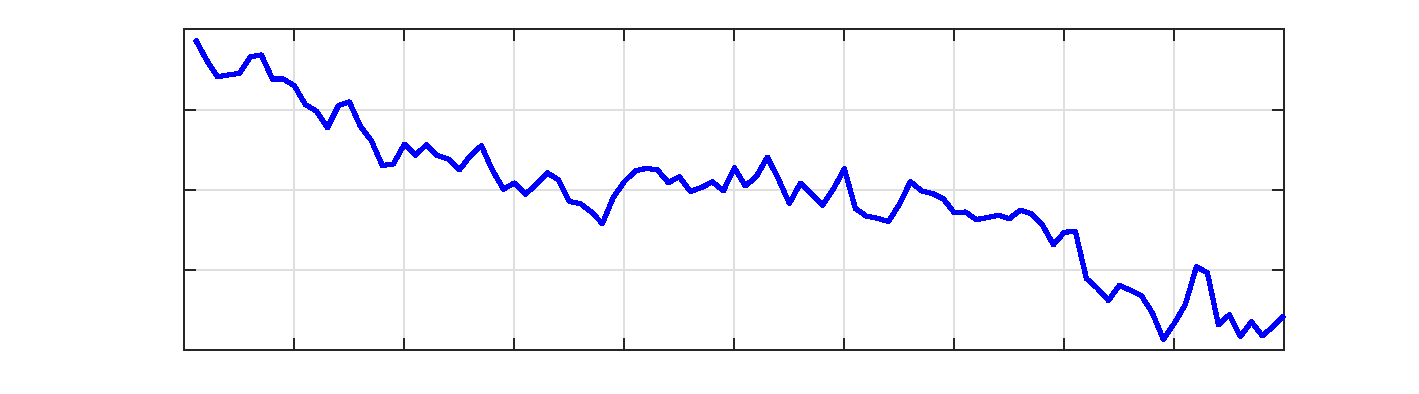
\includegraphics[trim={2.5cm 0 2cm 0}, clip,width=\columnwidth]{figures/gaussian.pdf}}

    \subfloat[Laplace: $p(x) = \frac{b}{2}e^{-b |x|}$]{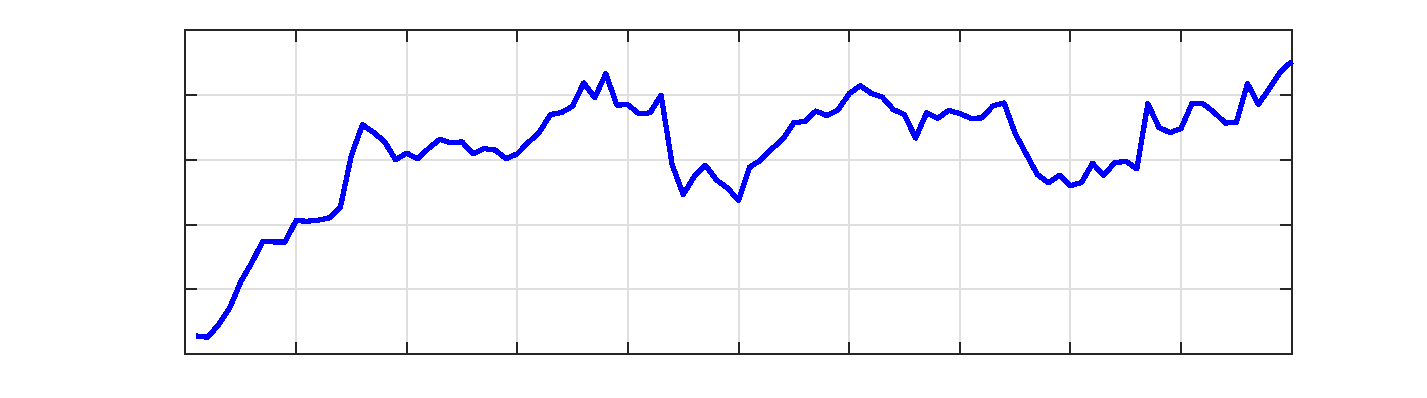
\includegraphics[trim={2.5cm 0 2cm 0}, clip,width=\columnwidth]{figures/laplace.pdf}}

    \subfloat[Bernoulli-Laplace: $p(x) = \lambda \delta(x) + (1-\lambda)\frac{b}{2}e^{-b |x|}$]{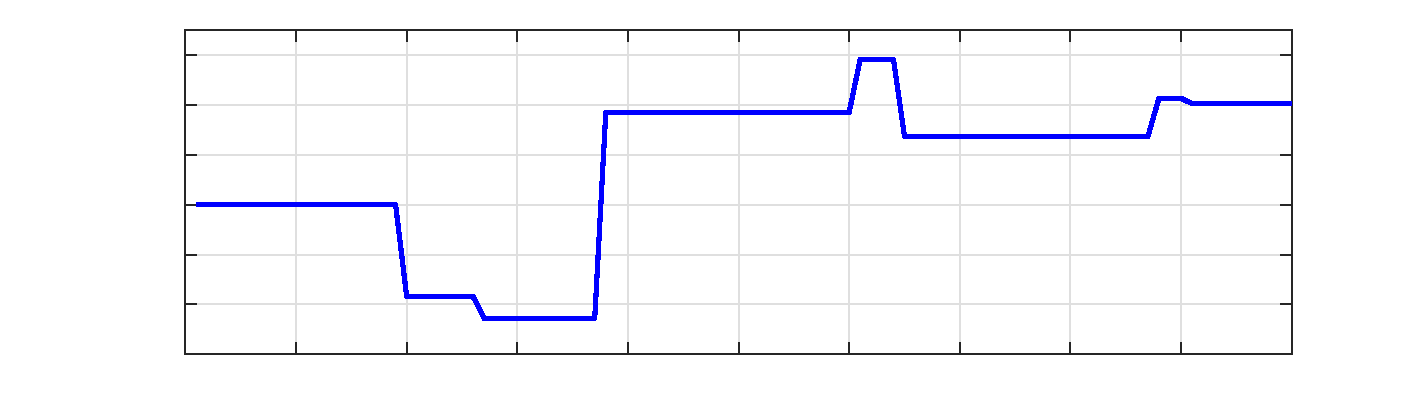
\includegraphics[trim={2.5cm 0 2cm 0}, clip,width=\columnwidth]{figures/bernoulli_laplace.pdf}}

    \subfloat[Cauchy: $p(x) = \frac{1}{\pi (1 + x^2)}$]{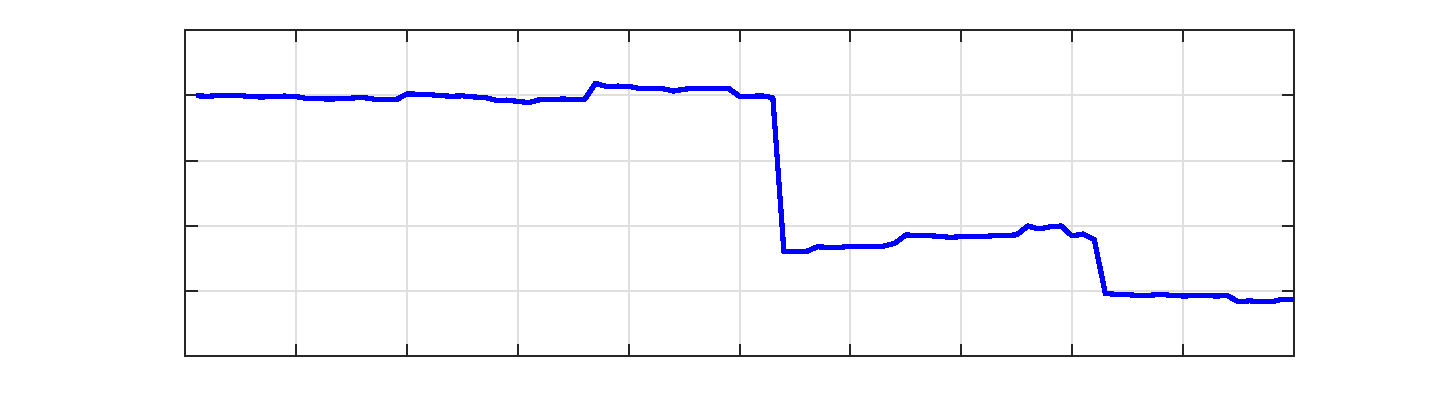
\includegraphics[trim={2.5cm 0 2cm 0}, clip,width=\columnwidth]{figures/cauchy.pdf}}

    \caption{Realizations of different L\'{e}vy processes}
    \label{fig:levy_processes}
\end{figure}

L\'{e}vy processes are closely linked to infinitely divisible (id) distributions. 

\begin{definition}[Infinite divisibility]
    A random variable $X$ is infinitely divisible (id) if, for any $N \in \N$, there exist independent and identically distributed (i.i.d.) random variables $X_1, \ldots, X_N$ such that $X = X_1 + \cdots + X_N$. 
\end{definition}

For any L\'{e}vy process $s$, the random variable $s(t)$, where $t>0$, is infinitely divisible, and its probability density function (pdf) is given by
\begin{equation}
    p_{s(t)}(x) = \int_{\R} \bigg(\int_{\R} p_{s(1)}(y) \mathrm{e}^{\mathrm{j} \omega y} \ud y \bigg)^t \mathrm{e}^{-\mathrm{j} \omega x} \frac{\ud \omega}{2\pi}. 
\end{equation}  
Conversely, for any id distribution with pdf $p_{\text{id}}$, it is possible to construct a L\'{e}vy process $s$ such that $p_{s(1)} = p_{\text{id}}$. Thus, there is a one-to-one correspondence between L\'{e}vy processes and id distributions \cite{ken1999levy}. 

The Gaussian distribution is the only member of the class of id distributions that is not sparse. The non-Gaussian members (\textit{e.g.,} Laplace, Bernoulli-Laplace, Student's t, symmetric-alpha-stable) are sparse in the sense that their pdfs exhibit a slower rate of decay at infinity \cite{amini2014sparsity}. Indeed, some of these sparse distributions have a mass at the origin in their pdf (\textit{e.g.,} Bernoulli-Laplace) and some of them are strongly compressible (\textit{e.g,} Student's t, symmetric-alpha-stable) \cite{amini2011compressibility}. Thus, the stochastic model of L\'{e}vy processes allows us to consider a variety of signals with varying degrees of sparsity. Some realizations of such processes are shown in Figure \ref{fig:levy_processes}.   


\subsection{Discrete Stochastic Model}
Now, we derive the pdf of the random vector $\M s = (s(k))_{k=1}^{K}$, which contains uniform samples of a L\'{e}vy process $s$. Consider the stationary increment process $u(t) = \{s(t) - s(t-1) : t \in \R^{+} \}$, whose first order pdf $p_u$ is the same as $p_{s(1)}$ and so is infinitely divisible. Its samples $\M u = (u(k))_{k=1}^{K}$ can be expressed as 
\begin{equation}\label{eq:discrete_innovation_model}
    \M u = \M D \M s,
\end{equation}
where $\M D$ is a finite-difference matrix of the form
\begin{equation}
    \M D = \begin{bmatrix}
        \phantom{-}1 & \phantom{-}0 & \phantom{-}0  & \phantom{-}\cdots  & \phantom{-}0\\
        -1 & \phantom{-}1 & \phantom{-}0  & \phantom{-}\cdots  & \phantom{-}0\\
        \phantom{-}0 & -1 & \phantom{-}1  & \phantom{-}\cdots  & \phantom{-}0\\
         &  & \phantom{-}\ddots & \phantom{-}\ddots &  \\
         \phantom{-}0 & \phantom{-}0  & \phantom{-}\cdots & -1 & \phantom{-}1
    \end{bmatrix}.
\end{equation}
Using \eqref{eq:discrete_innovation_model} and the fact that the increments are independent, we obtain the pdf of the discrete signal
\begin{equation}\label{eq:discrete_pdf}
    p_{\M s}(\M s) \propto \prod_{k = 1}^{K} p_{u}\big([\M D \M s]_k\big).
\end{equation}

Here, we would like to mention that \eqref{eq:discrete_innovation_model} can be alternatively written as
\begin{equation}\label{eq:gen_levy}
    [\M s]_k = \sum_{n=1}^{k} [\M u]_n, \ \ \ \ k = 1, \ldots, K,
\end{equation}
and this gives us a direct way to generate samples of any L\'{e}vy process. 


\section{Bayesian Inference}
So far, we have looked at the signal and measurement models that allow us to generate our ground-truth signals and simulate their noisy measurements for the chosen acquisition setup. Next, we focus on developing statistical estimators for the reconstruction problem at hand, which is to recover the signal $\M s$ from the measurements $\M y$.

In Bayesian inference, the goal is to characterize the posterior distribution $p_{\M s|\M y}$ and derive estimators based on it. Using Bayes' rule and $\eqref{eq:discrete_pdf}$, we get
\begin{align}\label{eq:posterior}
    p_{\M s|\M y}(\M s | \M y) &= \frac{p_{\M y|\M s}(\M y | \M s) p_{\M s}(\M s)}{\int_{\R^K} p_{\M y|\M s}(\M y | \M s) p_{\M s}(\M s) \ud \M s}  \nonumber \\
    &= \frac{1}{Z} \exp\bigg(-\frac{\|\M y - \M H \M s\|_{2}^{2}}{2 \sigma_{n}^{2}}\bigg) \prod_{k = 1}^{K} p_{u}\big([\M D \M s]_k\big),
\end{align}
where $Z$ is a normalizing constant.

\subsection{Maximum A Posteriori (MAP) Estimator}
The maximum a posteriori (MAP) estimator calculates the mode of the posterior distribution $p_{\M s| \M y}$ and is given by 
\begin{align} \label{eq:MAP}
    \widehat{\M s}_{\text{MAP}} &= \argmax_{\M s \in \R^K} \{p_{\M s | \M y}(\M s | \M y)\} \nonumber \\
&= \argmin_{\M s \in \R^K} \bigg\{\frac{1}{2 \sigma_{n}^{2}} \|\M y - \M H \M s\|_{2}^{2} + \sum_{k=1}^{K} \Phi_{u} \big([\M D \M s]_k \big) \bigg\},
\end{align}
where $\Phi_u(x) \triangleq -\log(p_u(x))$. The cost functional in \eqref{eq:MAP} consists of a quadratic data-fidelity term and a penalty term which penalizes undesirable solutions. The optimization task \eqref{eq:MAP} resembles the one formulated in the variational model-based methods. For instance, if $p_u$ is a Gaussian pdf, then the penalty term is $\|\M D \M s\|_{2}^{2}$ and we get the classical Tikhonov regularizer \cite{tikhonov1963}. However, if $p_u$ is a Laplace pdf, then we have a sparsity-promoting $\ell_1$-norm penalty term $\|\M D \M s\|_{1}$ which corresponds to the popular total variation (TV) regularizer \cite{rudin1992nonlinear}.

These MAP estimators can be computed efficiently with the help of iterative algorithms such as gradient descent, FISTA \cite{beck2009fast} and ADMM \cite{boyd2011distributed}.


\subsection{Minimum Mean Square Error (MMSE) Estimator}
The minimum mean square error (MMSE) estimator is given by
\begin{align}\label{eq:MMSE}
    \widehat{\M s}_{\text{MMSE}} &= \argmin_{{\M s'} \in \R^K} \bigg\{\int_{\R^K} \|\M s - \M s'\|_{2}^{2} \ p_{\M s|\M y}(\M s | \M y) \ud \M s \bigg\} \nonumber \\
&= \int_{\R^K} \M s \ p_{\M s|\M y}(\M s | \M y) \ud \M s,
\end{align}
which is the mean of the posterior distribution $p_{\M s|\M y}$. For a given set of measurements and a fixed stochastic model, the MMSE estimator is the optimal reconstructor in the mean-square-error sense and thus serves as the goldstandard in our benchmarking framework.

In the Gaussian case, the MMSE estimator is known to coincide with the MAP estimator and is straightforward to calculate \cite{kay1993fundamentals,unser2019biomedical}. However, in the non-Gaussian case, we need to numerically evaluate the integral in \eqref{eq:MMSE}, which is a difficult task in general. 


\section{Computing MMSE Estimators for Sparse L\'{e}vy Processes}
In this section, we present efficient methods to compute the MMSE estimator for sparse L\'{e}vy processes associated with the Laplace, Student's t and Bernoulli-Laplace distributions, which constitutes a key contribution of this paper.

\subsection{Markov Chain Monte Carlo (MCMC) Methods}
The MMSE estimator $\widehat{\M s}_{\text{MMSE}}$ involves the calculation of the integral \eqref{eq:MMSE}. The high-dimensionality of this integral makes its approximation by simple techniques such as uniform-grid-based Riemann sums infeasible. Instead, we can use Markov Chain Monte Carlo (MCMC) methods \cite{hastings1970monte, geyer1992practical,gilks1995markov,gamerman2006markov} for numerically approximating such integrals in a tractable manner.

MCMC methods are designed for generating random samples from nontrivial high-dimensional probability distributions. Broadly speaking, the idea in MCMC is to construct a Markov chain with the distribution that one wishes to draw samples from as its stationary distribution. The desired samples can be obtained by simulating the Markov chain and recording its states after convergence.

In order to compute the integral in \eqref{eq:MMSE}, we first generate samples $\{\M s^{(q)}\}_{q=1}^{Q}$ from $p_{\M s | \M y}$ using an MCMC method. We then approximate $\widehat{\M s}_{\text{MMSE}}$ by the estimate $\widehat{\M s}_{Q} = \frac{1}{Q} \sum_{q=1}^{Q} \M s^{(q)}$. Although the collected samples are correlated, the Markov Chain Central Limit Theorem \cite{gordin1978central} guarantees that $\widehat{\M s}_{Q}$ is a good approximation for $\widehat{\M s}_{\text{MMSE}}$ for large enough values of $Q$. 


\subsection{Gibbs Sampling}
In this work, we propose to use a MCMC method called Gibbs sampling \cite{geman1984stochastic,casella1992explaining} to generate samples $\{\M u^{(q)}\}_{q=1}^{Q}$ from the posterior distribution $p_{\M u | \M y}$. These can then be transformed using \eqref{eq:gen_levy} to obtain samples $\{\M D^{-1} \M u^{(q)}\}_{q=1}^{Q}$ from $p_{\M s | \M y}$. Here, we briefly describe the idea behind this algorithm. 

Let $x$ and $y$ be two random variables. Consider the task of generating samples from the joint distribution $p_{x, y}$. In this case, Gibbs sampling can be useful if it is computationally difficult to sample from the joint distribution directly but the conditional distributions $p_{x | y}$ and $p_{y |x}$ are easy to sample from. The steps involved in this method are presented in Algorithm \ref{alg:gibbs_sampling}. It can be shown that these yield a Markov chain whose stationary distribution is $p_{x, y}$ \cite{casella1992explaining}. In practice, we discard some of the initial samples (burn-in period) to allow the chain to converge. Moreover, quantities (expectation integrals) based on the marginal distributions $p_{x}$ and $p_{y}$ can be computed from the individual samples $\{x^{(q)}\}_{q=1}^{Q}$ and $\{y^{(q)}\}_{q=1}^{Q}$, respectively.  

\begin{algorithm}[t]
    \caption{Gibbs sampling}
    \begin{algorithmic}[1]
      \State \textbf{Input:} $Q$ (number of samples), $B$ (burn-in period)
      \State \textbf{Initialization:} $\big(x^{(0)}, y^{(0)}\big)$ 
      
      \For{$q = 1, \ldots, B+Q$}
        \State Generate $x^{(q)} \sim p_{x | y}\big(x | y^{(q-1)}\big)$
        \State Generate $y^{(q)} \sim p_{y | x}\big(y | x^{(q)}\big)$
      \EndFor

      \State \textbf{Output:} $\Big\{\big(x^{(q)}, y^{(q)}\big)\Big\}_{q=B+1}^{B+Q}$
    \end{algorithmic}
    \label{alg:gibbs_sampling}
  \end{algorithm}

Next, we present Gibbs samplers for Laplace, Student's t and Bernoulli-Laplace processes. There, the general strategy is to introduce an auxiliary vector $\M w$ and perform Gibbs sampling for the joint distribution $p_{\M u, \M w | \M y}$ \cite{tanner1987calculation,mira1997use}. The key is to choose $\M w$ such that the conditional distributions $p_{\M u | \M w, \M y}$ and $p_{\M w | \M u, \M y}$ can be sampled from in an efficient manner. 

Hereafter, we assume that the noise variance $\sigma_{n}^{2}$ and parameters of the signal model are known. However, if needed, it is possible to include their estimation within the Gibbs sampler.
 

\subsection{Laplace Process}
For Laplace processes, we adapt the approach that was developed in \cite{park2008bayesian}.  

The pdf for the Laplace distribution is 
\begin{equation}\label{eq:pdf_laplace}
    p_u(u) = \frac{b}{2}e^{-b |x|},
\end{equation}
where $b$ is the scale parameter. The density in \eqref{eq:pdf_laplace} can be expressed as a scale mixture of normal distributions \cite{andrews1974scale}, as 
\begin{equation}
    p_u(u) = \int_{\R} p_{u|w}(u|w) p_w(w) \ud w,
\end{equation}
where
\begin{equation}\label{eq:normal_laplace}
    p_{u|w}(u|w) = \frac{1}{\sqrt{2 \pi w}} \exp\bigg(-\frac{u^2}{2 w}\bigg)
\end{equation}
is the Gaussian pdf and  
\begin{equation}\label{eq:mixing_density_laplace}
    p_w(w) = \frac{b^2}{2}\exp\bigg(-\frac{b^2 w}{2}\bigg) \mathbbm{1}_{+}(w)
\end{equation}
is the exponential mixing pdf\footnote{The pdf of the exponential distribution is \begin{equation*} p(x) = (1/\lambda) \mathrm{e}^{-x/\lambda} \mathbbm{1}_{+}(x), \end{equation*} where $\lambda > 0$ is the scale parameter.}. This property allows us to define an auxiliary vector $\M w \in \R^K$, which has i.i.d entries following the distribution $p_w$ shown in \eqref{eq:mixing_density_laplace}, such that 
\begin{equation}\label{eq:aux_var_property_laplace}
    p_{\M u | \M w}(\M u | \M w) = \prod_{k=1}^{K} p_{u|w}\big([\M u]_k | [\M w]_k\big),
\end{equation}
where $p_{u|w}$ is shown in \eqref{eq:normal_laplace}.

Using the chain rule of probability (or the general product rule), the full joint distribution $p_{\M y, \M u, \M w}$ can be written as 
\begin{equation}\label{eq:full_joint_distribution_laplace}
    p_{\M y, \M u, \M w}(\M y, \M u, \M w) = p_{\M y | \M u}(\M y | \M u) p_{\M u | \M w}(\M u | \M w) p_{\M w}(\M w).
\end{equation}
Consequently, the distribution $p_{\M u, \M w | \M y}$ is of the form
\begin{align}\label{eq:conditional_joint_distribution_laplace}
    p_{\M u, \M w | \M y}(\M u, \M w | \M y) \propto \ &\exp\bigg(-\frac{1}{2 \sigma_n^2} \|\M y - \M A \M u \|_{2}^{2}\bigg) \nonumber \\
    &\times \ \prod_{k=1}^{K}[\M w]_k^{-\frac{1}{2}} \exp\bigg(-\frac{[\M u]_k^2}{2 [\M w]_k}\bigg) \nonumber \\
    &\times \ \prod_{k=1}^{K} \frac{b^2}{2}\exp\bigg(-\frac{b^2 [\M w]_k}{2}\bigg) \mathbbm{1}_{+}\big([\M w]_k\big),
\end{align}
where $\M A = \M H \M D^{-1}$. 

Based on \eqref{eq:conditional_joint_distribution_laplace}, the conditional distribution $p_{\M u | \M w, \M y}$ is then obtained as
\begin{align}\label{eq:conditional_u_laplace}
    p_{\M u | \M w, \M y}(\M u | \M w, \M y) \propto \ \exp\bigg(-\frac{1}{2}\bigg(&\frac{1}{\sigma_n^2}\|\M y - \M A \M u\|_{2}^{2} \nonumber \\
    & + \M u^{T} \M C(\M w) \M u \bigg) \bigg),
\end{align}
where $\M C(\M w)$ is a diagonal matrix with elements $\big([\M w]_k^{-1}\big)_{k=1}^{K}$. Specifically, $p_{\M u | \M w, \M y}$ is a multivariate Gaussian pdf with mean $\overline{\M u} = \sigma_n^{-2} \big(\sigma_n^{-2} \M A^{T} \M A + \M C(\M w)\big)^{-1}\M A^{T}\M y$ and covariance matrix $\overline{\M R} = \big(\sigma_n^{-2} \M A^{T} \M A + \M C(\M w)\big)^{-1}$. There exist several methods for efficiently generating samples from a multivariate Gaussian density \cite{rue2001fast,vono2022high}.

The other conditional distribution $p_{\M w | \M u, \M y}$ is
\begin{equation}
    p_{\M w | \M u, \M y}(\M w | \M u, \M y) \propto \prod_{k=1}^{K} p_{w|u, \M y}\big([\M w]_k|[\M u]_k, \M y\big),
\end{equation}
where
\begin{align}\label{eq:conditional_w_laplace}
    p_{w | u, \M y}\big(w | u, \M y\big) \propto \ &\exp\bigg(-\frac{1}{2}\bigg(\frac{u^2}{w} + b^2 w\bigg)\bigg) \nonumber \\
    &\times \ w^{-\frac{1}{2}} \mathbbm{1}_{+}(w)
\end{align}
belongs to the family of generalized inverse Gaussian distributions\footnote{The pdf of the generalized inverse Gaussian distribution is \begin{equation*} p(x) = \frac{(\lambda_1/\lambda_2)^{p/2}}{2K_p(\sqrt{\lambda_1 \lambda_2})}x^{p-1} \mathrm{e}^{-(\lambda_1 x + \lambda_2/x)/2} \mathbbm{1}_{+}(x), \end{equation*} where $K_p$ is a modified Bessel function of the second kind, $\lambda_1 > 0$, $\lambda_2 > 0$ and $p \in \R$.} with $\lambda_1 = b^2$, $\lambda_2 = u^2$ and $p = 0.5$. We use the method proposed in \cite{devroye2014random} to draw samples from the pdf in \eqref{eq:conditional_w_laplace}.

To summarize, at each iteration $q$ of the constructed blocked Gibbs sampler, we generate $\M u^{(q)} \sim p_{\M u | \M w,\M y}\big(\M u | \M w^{(q-1)}, \M y\big)$ and $[\M w^{(q)}]_k \sim p_{w | u,\M y}\big(w | [\M u^{(q)}]_k,\M y \big)$ for all $k\in \{1,\ldots,K\}$. The collected samples $\{\M u^{(q)}\}_q$ follow the desired distribution $p_{\M u | \M y}$.

% \begin{algorithm}[t]
%     \caption{Gibbs sampler for Laplace processes}
%     \begin{algorithmic}[1]
%       \State \textbf{Input:} $\M y$, $\M H$, $\M D$, $\sigma_n^2$, $b$, $Q$ (number of samples), $B$ (burn-in period)
%       \State \textbf{Initialization:} $\M u^{(0)}, \M w^{(0)}$, $\M A = \M H \M D^{-1}$ 
      
%       \For{$q = 1, \ldots, B+Q$}
%         \State Generate $\M u^{(q)} \sim p_{\V U | \V W,\V Y}\big(\M u | \M w^{(q-1)}, \M y\big)$ where $p_{\V U | \V W,\V Y}$ is a Gaussian distribution with mean 

%         \State Generate $[\M w]_k^{(q)} \sim p_{W | \V U,\V Y}\big(\M w | \M u^{(q)},\M y \big)$ for all $k\in \{1,\ldots,K\}$, where 
%       \EndFor

%       \State \textbf{Output:} $\Big\{\Big(x_1^{(q)}, x_2^{(q)}, x_3^{(q)}\Big)\Big\}_{q=B+1}^{B+Q}$
%     \end{algorithmic}
%     \label{alg:gibbs_sampling_laplace}
%   \end{algorithm}


% \begin{algorithm}[t]
%     \caption{Gibbs sampler for Student's t processes}
%     \begin{algorithmic}[1]
%       \State \textbf{Input:} $Q$ (number of samples), $B$ (burn-in period)
%       \State \textbf{Initialization:} $\Big(x_1^{(0)}, x_2^{(0)}, x_3^{(0)}\Big)$ 
      
%       \For{$q = 1, \ldots, B+Q$}
%         \State Generate $x_1^{(q)} \sim p_{X_1 | X_2,X_3}\Big(x_1 \ | \ x_2^{(q-1)}, \ x_3^{(q-1)}\Big)$
%         \State Generate $x_2^{(q)} \sim p_{X_2 | X_1,X_3}\Big(x_2 \ | \ x_1^{(q)}, \ x_3^{(q-1)}\Big)$
%         \State Generate $x_3^{(q)} \sim p_{X_3 | X_1,X_2}\Big(x_3 \ | \ x_1^{(q)}, \ x_2^{(q)}\Big)$
%       \EndFor

%       \State \textbf{Output:} $\Big\{\Big(x_1^{(q)}, x_2^{(q)}, x_3^{(q)}\Big)\Big\}_{q=B+1}^{B+Q}$
%     \end{algorithmic}
%     \label{alg:gibbs_sampling_student}
%   \end{algorithm}


\subsection{Student's t Process}
The case of Student's t processes can be handled by adapting the method shown in \cite{fevotte2006bayesian}, which is in fact similar to the one we described for Laplace processes. 


The Student's t pdf is given by 
\begin{equation}\label{eq:pdf_student}
    p_u(u) = \frac{\Gamma(\frac{\alpha+1}{2})}{\Gamma\big(\frac{\alpha}{2}\big)}\frac{1}{\sqrt{\pi}(1 + u^2)^{\frac{\alpha+1}{2}}},
\end{equation}
where $\alpha$ is the number of degrees of freedom and controls the tail of the distribution, and $\Gamma$ denotes the gamma function. It can also be expressed as 
\begin{equation}
    p_u(u) = \int_{\R} p_{u|w}(u|w) p_w(w) \ud w,
\end{equation}
where
\begin{equation}\label{eq:normal_student}
    p_{u|w}(u|w) = \sqrt{\frac{w}{2 \pi}} \exp\bigg(- \frac{w u^2}{2}\bigg)
\end{equation}
is a Gaussian pdf and  
\begin{equation}\label{eq:mixing_density_student}
    p_w(w) = \frac{(0.5)^{\frac{\alpha}{2}}}{\Gamma(\frac{\alpha}{2})}w^{\frac{\alpha}{2}-1} \exp{\Big(-\frac{w}{2}\Big)} \ \mathbbm{1}_{+}(w)
\end{equation}
is the pdf of a gamma\footnote{The pdf of the gamma distribution is \begin{equation*} p(x) = \frac{1}{\lambda_2^{\lambda_1} \Gamma(\lambda_1)}x^{\lambda_1-1}e^{-x/\lambda_2} \mathbbm{1}_{+}(x), \end{equation*} where $\lambda_1 > 0$ and $\lambda_2 > 0$.} distribution. Again, we introduce an auxiliary vector $\M w \in \R^K$, whose i.i.d entries follow $p_w$ defined in \eqref{eq:mixing_density_student}, such that 
\begin{equation}\label{eq:aux_var_property_student}
    p_{\M u | \M w}(\M u | \M w) = \prod_{k=1}^{K} p_{u|w}\big([\M u]_k | [\M w]_k\big),
\end{equation}
where $p_{u|w}$ is defined in \eqref{eq:normal_student}.

Here, the distribution $p_{\M u, \M w | \M y}$ is given by
\begin{align}\label{eq:conditional_joint_distribution_student}
    p_{\M u, \M w | \M y}(\M u, \M w | \M y) \propto \ &\exp\bigg(-\frac{1}{2 \sigma_n^2} \|\M y - \M A \M u \|_{2}^{2}\bigg) \nonumber \\
    &\times \ \prod_{k=1}^{K}[\M w]_k^{\frac{1}{2}} \exp\bigg(-\frac{[\M w]_k [\M u]_k^2}{2}\bigg) \nonumber \\
    &\times \ \prod_{k=1}^{K} [\M w]_k^{\frac{\alpha}{2} - 1} \exp{\bigg(-\frac{[\M w]_k}{2}\bigg)} \mathbbm{1}_{+}\big([\M w]_k\big),
\end{align}
where $\M A = \M H \M D^{-1}$. 

Now, the conditional distribution $p_{\M u | \M w, \M y}(\M u | \M w, \M y)$ turns out to be
\begin{align}\label{eq:conditional_u_student}
    p_{\M u | \M w, \M y}(\M u | \M w, \M y) \propto \ \exp\bigg(-\frac{1}{2}\bigg(&\frac{1}{\sigma_n^2}\|\M y - \M A \M u\|_{2}^{2} \nonumber \\
    & + \M u^{T} \M C'(\M w) \M u \bigg) \bigg),
\end{align}
where $\M C'(\M w)$ is a diagonal matrix with entries $\big([\M w]_k\big)_{k=1}^{K}$. Similar to the Laplace case, $p_{\M u | \M w, \M y}$ is a multivariate Gaussian density with mean $\overline{\M u} = \sigma_n^{-2} \big(\sigma_n^{-2} \M A^{T} \M A + \M C'(\M w)\big)^{-1}\M A^{T}\M y$ and covariance matrix $\overline{\M R} = \big(\sigma_n^{-2} \M A^{T} \M A + \M C'(\M w)\big)^{-1}$. 

The distribution $p_{\M w | \M u, \M y}$ is again separable and takes the form 
\begin{equation}
    p_{\M w | \M u, \M y}(\M w | \M u, \M y) \propto \prod_{k=1}^{K} p_{w|u, \M y}\big([\M w]_k|[\M u]_k, \M y\big),
\end{equation}
where
\begin{align}\label{eq:conditional_w_student}
    p_{w | u, \M y}\big(w | u, \M y\big) \propto \ &\exp\bigg(-\frac{(1 + u)^2 w}{2}\bigg) \nonumber \\
    &\times \ w^{\frac{\alpha-1}{2}} \mathbbm{1}_{+}(w).
\end{align}
is a gamma distribution with $\lambda_1 = \frac{\alpha + 1}{2}$ and $\lambda_2 = \frac{2}{(1 + u)^2}$, which can be sampled from easily.


\subsection{Bernoulli-Laplace Process}
In \cite{ge2011enhanced}, Gibbs sampling schemes have been designed for a deconvolution problem where the underlying signal is an i.i.d spike train following the Bernoulli-Gaussian distribution. Unfortunately, the Bernoulli-Gaussian distribution is not infinitely divisible and so is not compatible with our framework of L\'{e}vy processes. Thus, we build upon their method and develop a novel Gibbs sampler for Bernoulli-Laplace processes.  


The Bernoulli-Laplace pdf is
\begin{equation}\label{eq:pdf_bl}
    p_u(u) = \lambda \delta(u) + (1-\lambda)\frac{b}{2}e^{-b |u|},  
\end{equation}
where $\lambda \in (0,1)$ denotes the mass probability at the origin and $b$ is a scale parameter. We can also represent this density as
\begin{equation}
    p_u(u) = \int_{\R} \bigg(\sum_{v=0}^{1} p_{u|v, w}(u|v, w) p(v) \bigg) p(w) \ud w,
\end{equation}
where
\begin{equation}\label{eq:bernoulli_bl}
    p_{v}(v) = (\lambda)^{1-v}(1-\lambda)^{v} \ \ \text{for } v = \{0,1\}
\end{equation}
is a Bernoulli pdf,
\begin{equation}\label{eq:bernoulli_exponential}
    p_{w}(w) = \frac{b^2}{2}\exp\bigg(-\frac{b^2 w}{2}\bigg) \mathbbm{1}_{+}(w)
\end{equation}
is an exponential pdf, and $p_{u|v, w}$ is defined such that
\begin{align}
    &p_{u|v, w}(u|v=0, w) = \delta(u) \label{eq:dirac_bl}\\
    &p_{u|v, w}(u|v=1, w) = \frac{1}{\sqrt{2 \pi w}} \exp\bigg(-\frac{u^2}{2 w}\bigg) \label{eq:gaussian_bl}.
\end{align}
Based on this representation, we introduce two independent auxiliary vectors $\M v \in \R^K$ and $\M w \in \R^K$. Their elements are i.i.d and follow the distributions $p_{v}$ and $p_{w}$, as defined in \eqref{eq:bernoulli_bl} and \eqref{eq:bernoulli_exponential}, respectively. Further, these vectors satisfy
\begin{equation}\label{eq:aux_var_property_bl}
    p_{\M u | \M v, \M w}(\M u | \M v, \M w) = \prod_{k=1}^{K}p_{u|v, w}\big([\M u]_k | [\M v]_k, [\M w]_k\big),
\end{equation}
where $p_{u|v, w}$ is defined in \eqref{eq:dirac_bl} and \eqref{eq:gaussian_bl}.

Here, the full joint distribution $p_{\M y, \M u, \M v, \M w}$ is given by 
\begin{align}
    p_{\M y, \M u, \M v, \M w}(\M y, \M u, \M v, \M w) = \ &p_{\M y | \M u}(\M y | \M u) p_{\M u | \M v, \M w}(\M u | \M v, \M w) \nonumber \\ 
    &\times \ p_{\M v}(\M v) p_{\M w}(\M w).
\end{align}
As a result, the distribution $p_{\M u, \M v, \M w|\M y}$ takes the form
\begin{align}\label{eq:conditional_joint_distribution_bl}
    p_{\M u, \M v, \M w | \M y}(\M u, \M v, \M w | \M y&) \ \propto \ \exp\bigg(-\frac{1}{2 \sigma_n^2} \|\M y - \M A \M u \|_{2}^{2}\bigg) \nonumber \\
    &\times \ \prod_{k=1}^{K}p_{u|v, w}\big([\M u]_k | [\M v]_k, [\M w]_k\big) \nonumber \\
    &\times \ \prod_{k=1}^{K} \lambda^{1-[\M v]_k}(1-\lambda)^{[\M v]_k} \nonumber \\
    &\times \ \prod_{k=1}^{K} \frac{b^2}{2}\exp\bigg(-\frac{b^2 [\M w]_k}{2}\bigg) \mathbbm{1}_{+}([\M w]_k),
\end{align}
where $\M A = \M H \M D^{-1}$. 

Before deriving the conditional distributions, we introduce some notations to make the exposition clearer. For any binary vector $\M q \in \R^K$, let $\mathcal{I}_{\M q, 0}$ and $\mathcal{I}_{\M q, 1}$ denote sets of indices such that $[\M q]_k = 0$ for $k \in \mathcal{I}_{\M q, 0}$ and $[\M q]_k = 1$ for $k \in \mathcal{I}_{\M q, 1}$. Further, let $\M A(\M q)$ be the matrix constructed by taking the columns of $\M A$ corresponding to the indices in $\mathcal{I}_{\M q, 1}$. We then define the matrix $\M B(\M q, \M r) = \sigma_n^{2} \M I + \M A(\M q) \M C''(\M q, \M r) \M A(\M q)^{T}$, where $\M r \in \R^K$ is a vector with positive entries and $\M C''(\M q, \M r)$ is a diagonal matrix with entries $([\M r]_k)_{k \in \mathcal{I}_{\M q, 1}}$. Here, we also introduce the quantity $\M q_{(-k)} \in \R^{K-1}$ that contains all the entries of $\M q$ except the $k^{\text{th}}$ one, that is, $\M q_{(-k)} = ([\M q]_{1}, \ldots, [\M q]_{k-1}, [\M q]_{k+1}, \ldots, [\M q]_{K})^T$. Lastly, for $q = \{0,1\}$, we define the vector $\M q_{(-k)}^{q} \in \R^{K}$ such that $\M q_{(-k)}^{q} = ([\M q]_{1}, \ldots, [\M q]_{k-1}, q, [\M q]_{k+1}, \ldots, [\M q]_{K})^T$. 

First, we look at the conditional distribution $p_{\M u | \M v, \M w, \M y}$. From \eqref{eq:dirac_bl} and \eqref{eq:conditional_joint_distribution_bl}, it can be deduced that any sample from $p_{\M u | \M v, \M w, \M y}$ takes the value of zero at the indices in $\mathcal{I}_{\M v, 0}$. If we define $\M u_1 = ([\M u]_k)_{k \in \mathcal{I}_{\M v, 1}}$, then we get
\begin{align}\label{eq:conditional_u_bl}
    p_{\M u_1 | \M v, \M w, \M y}(\M u_1 | \M v, \M w, \M y) \propto  \exp\bigg(\hspace{-0.1cm}&-\frac{1}{2}\bigg(\frac{1}{\sigma_n^2}\|\M y - \M A(\M v) \M u_1\|_{2}^{2} \nonumber \\
    & + \M u_1^{T} \M C''(\M v, \M w) \M u_1 \bigg) \bigg).
\end{align}
Thus, $p_{\M u_1 | \M v, \M w, \M y}$ is a multivariate Gaussian density with mean $\overline{\M u_1} = \sigma_n^{-2} \big(\sigma_n^{-2} \M A(\M v)^{T} \M A(\M v) + \M C''(\M v, \M w)\big)^{-1}\M A(\M v)^{T}\M y$ and covariance matrix $\overline{\M R} = \big(\sigma_n^{-2} \M A(\M v)^{T} \M A(\M v) + \M C''(\M v, \M w)\big)^{-1}$.

The conditional distribution $p_{\M w | \M u, \M v, \M y}$ is of the form
\begin{align}
    p_{\M w | \M u, \M v, \M y}(\M w | \M u, \M v, &\M y) \propto \prod_{k=1}^{K} p_{w|u, v, \M y}\big([\M w]_k|[\M u]_k, [\M v]_k, \M y \big), 
\end{align} 
where $p_{w|u, v, \M y}$ is given by
\begin{equation}\label{eq:conditional_w2_bl_exp}
    p_{w|u, v, \M y}(w|u, v=0, \M y) \propto \frac{b^2}{2}\exp\bigg(-\frac{b^2 w}{2}\bigg) \mathbbm{1}_{+}(w)
\end{equation}
\begin{align}\label{eq:conditional_w2_bl_gig}
    p_{w|u, v, \M y}(w|u, v=1, \M y) \propto \ &\exp\bigg(-\frac{1}{2}\bigg(\frac{u^2}{w} + b^2 w\bigg)\bigg) \nonumber \\
    &\times \ w_2^{-\frac{1}{2}} \mathbbm{1}_{+}(w).
\end{align}
The densities in \eqref{eq:conditional_w2_bl_exp} and \eqref{eq:conditional_w2_bl_gig} correspond to the exponential distribution with $\lambda = \frac{2}{b^2}$ and the generalized inverse Gaussian distribution with $\lambda_1 = b^2$, $\lambda_2 = u^2$ and $p = 0.5$.

In the standard blocked Gibbs sampler, we would draw samples from the conditional distribution $p_{\M v | \M u, \M w, \M y}$. However, as pointed out in \cite{ge2011enhanced}, this sampler would have a tendency to get stuck in certain configurations of $\M v$. Therefore, inspired by the work in \cite{ge2011enhanced}, we instead consider sampling from the marginalized conditional distribution of $[\M v]_k$ in a sequential manner. More specifically, at each iteration $q$, we draw $[\M v^{(q)}]_k$ from the distribution $p_{[\M v]_k | \M v_{(-k)}, \M w, \M y}\big(v | \M v_{(-k)}^{(q)}, \M w^{(q)}, \M u^{(q-1)}\big)$, where $\M v_{(-k)}^{(q)} = \big([\M v^{(q)}]_{1}, \ldots, [\M v^{(q)}]_{k-1}, [\M v^{(q-1)}]_{k+1}, \ldots, [\M v^{(q-1)}]_{K} \big)$ and $k \in \{1, \ldots, K\}$.

The marginalized posterior distribution $p_{\M v, \M w | \M y}$ is given by 
\begin{align}\label{eq:marginal_integral_bl_tmp}
    p_{\M v, \M w | \M y}(\M v, \M w | \M y) \propto p_{\M y|\M v, \M w}(\M y|\M v, \M w) p_{\M v}(\M v) p_{\M w}(\M w), 
\end{align}
where 
\begin{equation}\label{eq:marginal_integral_bl}
    p_{\M y|\M v, \M w}(\M y|\M v, \M w) = \hspace{-0.15cm} \int_{\R^K} p_{\M y|\M u, \M v, \M w}(\M y | \M u, \M v, \M w) p_{\M u|\M v, \M w}(\M u|\M v, \M w) \ud \M u.
\end{equation}
It can be shown that evaluating \eqref{eq:marginal_integral_bl_tmp} and \eqref{eq:marginal_integral_bl} leads to
\begin{align}\label{eq:marginalized_posterior_distribution_bl}
    p_{\M v, \M w | \M y}(\M v, \M w | \M y) \propto& \ |\M B(\M v, \M w)|^{-\frac{1}{2}} \exp\bigg(-\frac{1}{2} \M y^{T} \M B(\M v, \M w)^{-1} \M y \bigg) \nonumber \\
    &\times \ \prod_{k=1}^{K} \lambda^{1-[\M v]_k}(1-\lambda)^{[\M v]_k} \nonumber \\
    &\times \ \prod_{k=1}^{K} \frac{b^2}{2}\exp\bigg(-\frac{b^2 [\M w]_k}{2}\bigg) \mathbbm{1}_{+}([\M w]_k).
\end{align}
From \eqref{eq:marginalized_posterior_distribution_bl}, we see that $p_{[\M v]_k | \M v_{(-k)}, \M w, \M y}$ is a Bernoulli distribution with
\begin{align*}
    p_{[\M v]_k | \M v_{(-k)}, \M w, \M y}(v|\M v_{(-k)}, \M w, \M y) = \hspace{4cm}
\end{align*}
\begin{align} 
    \bigg(1 + \exp\bigg(-\frac{1}{2}\Big(&h\big(1-v; \M v_{(-k)}, \M w, \M y\big) \nonumber \\
    &- h\big(v; \M v_{(-k)}, \M w, \M y\big)\Big)\bigg)\bigg)^{-1},
\end{align}
where
\begin{align}
    h\big(v; \M v_{(-k)}, \M w, \M y\big) =& \ \M y^{T} \M B\big(\M v_{(-k)}^{v}, \M w\big)^{-1} \M y \nonumber \\
    &+ \log\big(|\M B\big(\M v_{(-k)}^{v}, \M w\big)|\big) \nonumber \\
    &+ 2 v \log\Big(\frac{1-\lambda}{\lambda}\Big).
\end{align}

To summarize, in each iteration $q$ of the above-described sampler, we generate $\M w^{(q)} \sim p_{\M w | \M u, \M v, \M y}\big(\M w | \M u^{(q-1)}, \M v^{(q-1)}, \M y\big)$, $[\M v^{(q)}]_k \sim p_{[\M v]_k | \M v_{(-k)}, \M w, \M y}\big(v | \M v_{(-k)}^{(q)}, \M w^{(q)}, \M u^{(q-1)}\big)$ for all $k$ and $\M u^{(q)} \sim p_{\M u | \M v, \M w,\M y}\big(\M u | \M v^{(q)}, \M w^{(q)}, \M y\big)$. This particular order of updates is important as it yields a partially collapsed Gibbs sampler \cite{van2008partially} where the stationary distribution is still $p_{\M u, \M v, \M w | \M y}$.   


\section{Experimental Results}
In this section, we present some numerical experiments to illustrate the potential of our framework.

\subsection{Methods}
In our experiments, we benchmark the performance of a CNN-based direct nonlinear reconstruction scheme on deconvolution and Fourier sampling problems with L\'{e}vy processes associated with the Bernoulli-Laplace and Student's t distributions, respectively. This method involves training a CNN as a regression model that maps an initial low-quality reconstruction $\widehat{\M s}_{0}$ to a high-quality one $\widehat{\M s}_{\text{CNN}}$ \cite{jin2017deep,chen2017low,hyun2018deep, monakhova2019learned,perdios2020cnn}. The architecture of our CNN is based on the well-known denoising network DnCNN \cite{zhang2017beyond} and is described in Figure \ref{fig:CNN_architecture} and Table \ref{table:conv_layers}. Given a dataset $\{\M s_{m}, \M y_m\}_{m=1}^{M_T}$ of ground-truth signals and their corresponding measurements, we train the model by minimizing the MSE loss function 
\begin{equation}
    \mathcal{L}(\V \theta) = \frac{1}{M_T} \sum_{m=1}^{M_T} \|\M s_{m} - \widehat{\M s}_{\text{CNN}}\big(\V \theta; \widehat{\M s}_{0}(\M y_m)\big) \|_{2}^{2},
\end{equation}
where $\V \theta$ represents the learnable parameters of the network, with the help of the ADAM optimizer \cite{kingma2014adam}. This scheme is implemented in PyTorch.

\begin{figure}[t]
    \centering
    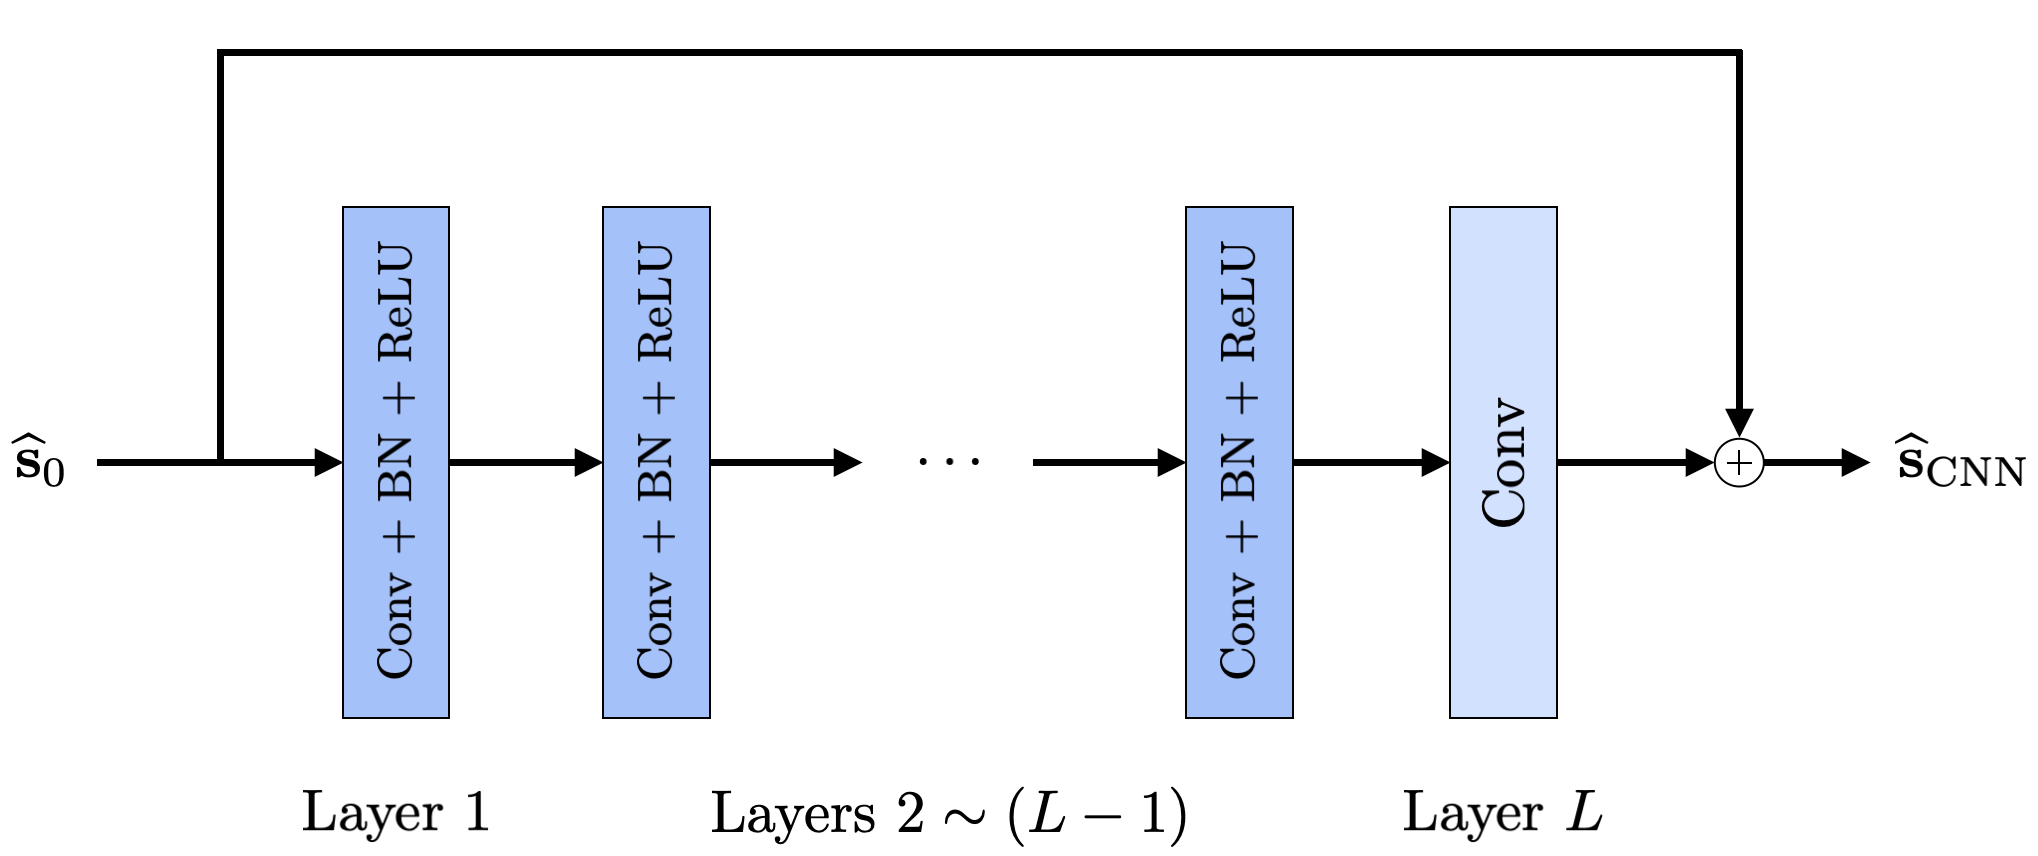
\includegraphics[width=\linewidth]{figures/cnn_architecture.png}
    \caption{Architecture of the CNN, where BN denotes the batch normalization operation.}
    \label{fig:CNN_architecture}
\end{figure}
        
\begin{table}[t]
\caption{Convolution Layers}
\label{table:conv_layers}
\setlength{\tabcolsep}{3pt}
\renewcommand{\arraystretch}{1.5}
\centering
\begin{tabular}[c]{c| c | c | c}
\hline \hline
Layer  & Filter size & {Input channels} & Output channels  \\ \hline 
1 & $F \times 1$ & $1$ & $C$ \\
2 $\sim$ ($L-1$) & $F \times 1$ & $C$ & $C$  \\ 
$L$ & $F \times 1$ & $C$ & $1$  \\ \hline \hline 
\end{tabular}
\end{table}

We compare the CNN-based method with the MMSE estimators for the underlying signal models and with the model-based techniques 
\begin{equation}\label{eq:est_l2}
    \widehat{\M s}_{\ell_2} = \argmin_{\M s \in \R^K} \Big\{\|\M y - \M H \M s\|_{2}^{2} + \tau \|\M D \M s\|_{2}^{2} \Big\},
\end{equation}
\begin{equation}\label{eq:est_l1}
    \widehat{\M s}_{\ell_1} = \argmin_{\M s \in \R^K} \Big\{\|\M y - \M H \M s\|_{2}^{2} + \tau \|\M D \M s\|_{1} \Big\},
\end{equation}
and
\begin{equation}\label{eq:est_log}
    \widehat{\M s}_{\text{log}} = \argmin_{\M s \in \R^K} \Big\{\|\M y - \M H \M s\|_{2}^{2} + \tau \sum_{k=1}^{K} \log \Big(1 + \big([\M D \M s]_k\big)^{2}\Big) \Big\},
\end{equation}
where $\tau \in \R_{+}$. Equations \eqref{eq:est_l2}, \eqref{eq:est_l1} and \eqref{eq:est_log} resemble the MAP estimators of Gaussian, Laplace and Student's t L\'{e}vy processes, respectively. However, unlike the MAP estimators, these include an adjustable hyperparameter $\tau$ which we tune to optimize their performance. This makes the benchmark harder for the CNN-based method. The $\ell_2$ estimator can be computed in a direct manner due to the availability of its closed-form expression
\begin{equation}
    \widehat{\M s}_{\ell_2} = \big(\M H^{T} \M H + \tau \M D^{T} \M D \big)^{-1} \M H^{T} \M y.
\end{equation}
On the other hand, the $\ell_1$ and log estimators are computed using ADMM. Since the cost functional in \eqref{eq:est_log} is non-convex, we initialize ADMM for $\widehat{\M s}_{\text{log}}$ with $\widehat{\M s}_{\ell_1}$ so that it can reach a better local minima. The MMSE and variational estimators are implemented in MATLAB using GlobalBioIm \cite{soubies2019pocket}, a library for solving inverse problems.



\subsection{Deconvolution}
We first consider a deconvolution problem where the signal vector $\M s \in \R^{100}$ contains samples of a L\'{e}vy process whose increments follow the Bernoulli-Laplace distribution. As shown in Section \ref{sec:deconv_forward}, the system matrix $\M H$ for this case turns out to be a discrete convolution-like matrix. Accordingly, we construct $\M H: \R^{100} \rightarrow \R^{88}$ such that
\begin{equation}
    \M H = \begin{bmatrix}
        [\M h]_{13} & \cdots & [\M h]_1 & 0  & \cdots & 0 \\
        0 & \ddots & & \ddots & \ddots & \vdots \\ 
        \vdots & \ddots & \ddots & & \ddots & 0 \\
        0 & \cdots & 0 & [\M h]_{13} & \cdots & [\M h]_1
        \end{bmatrix},
\end{equation}
where $\M h \in \R^{13}$ consists of samples of a truncated Gaussian PSF with variance $\sigma_{0}^{2} = 4$. The Bernoulli-Laplace pdf \eqref{eq:pdf_bl} is characterized by the parameters $\lambda$ and $b$, where $\lambda$ determines the mass probability at the origin and $b$ represents the scale of the Laplace component. For chosen values of $\lambda, b$ and the AWGN variance $\sigma_n^{2}$, we generate training, validation and test datasets consisting of $50,000$, $1,000$ and $1,000$ pairs of ground-truth signals and their noisy measurements, respectively. 

For the CNN-based approach, we set $F=3$, $C=32$ and $L=10$, and we choose the initial low-quality reconstruction to be $\widehat{\M s}_{0}(\M y) = \M H^{T} \M y$. The CNN is trained for $500$ epochs with a learning rate of $10^{-4}$ and a batch size of $128$. For each variational method, the same regularization parameter $\tau$ is used for the entire test dataset. This particular value of $\tau$ is the one that yields the lowest collective MSE for the validation dataset. For the Gibbs-sampling-based MMSE estimator, we set the number of samples as $Q=10,000$ and the burn-in period as $B=3,000$.

We perform the above-described deconvolution experiment for $\lambda \in \{ 0.6, 0.7, 0.8, 0.9 \}$. In each case, the scale parameter is set to $b=1$ and $\sigma_n^{2}$ is chosen such that the (average) measurement SNR is around $30$ dB. The results for the test dataset are shown in Figure \ref{fig:deconvolution_bl}.

The sparsity-promoting $\ell_1$ estimator, which corresponds to the popular TV regularization, is known to be well-suited for the piecewise-constant Bernoulli-Laplace L\'{e}vy processes. As the value of $\lambda$ increases, these signals become sparser and exhibit fewer jumps. Consequently, we observe that the $\ell_1$ estimator performs considerably better than the $\ell_2$ estimator. However, despite being a good fit, there is still some gap between the MSE attained by the $\ell_1$ and MMSE estimators. Remarkably, the CNN-based method consistently outperforms the TV-regularized method and achieves a near-optimal MSE.



\begin{figure}[t]
    \centering
    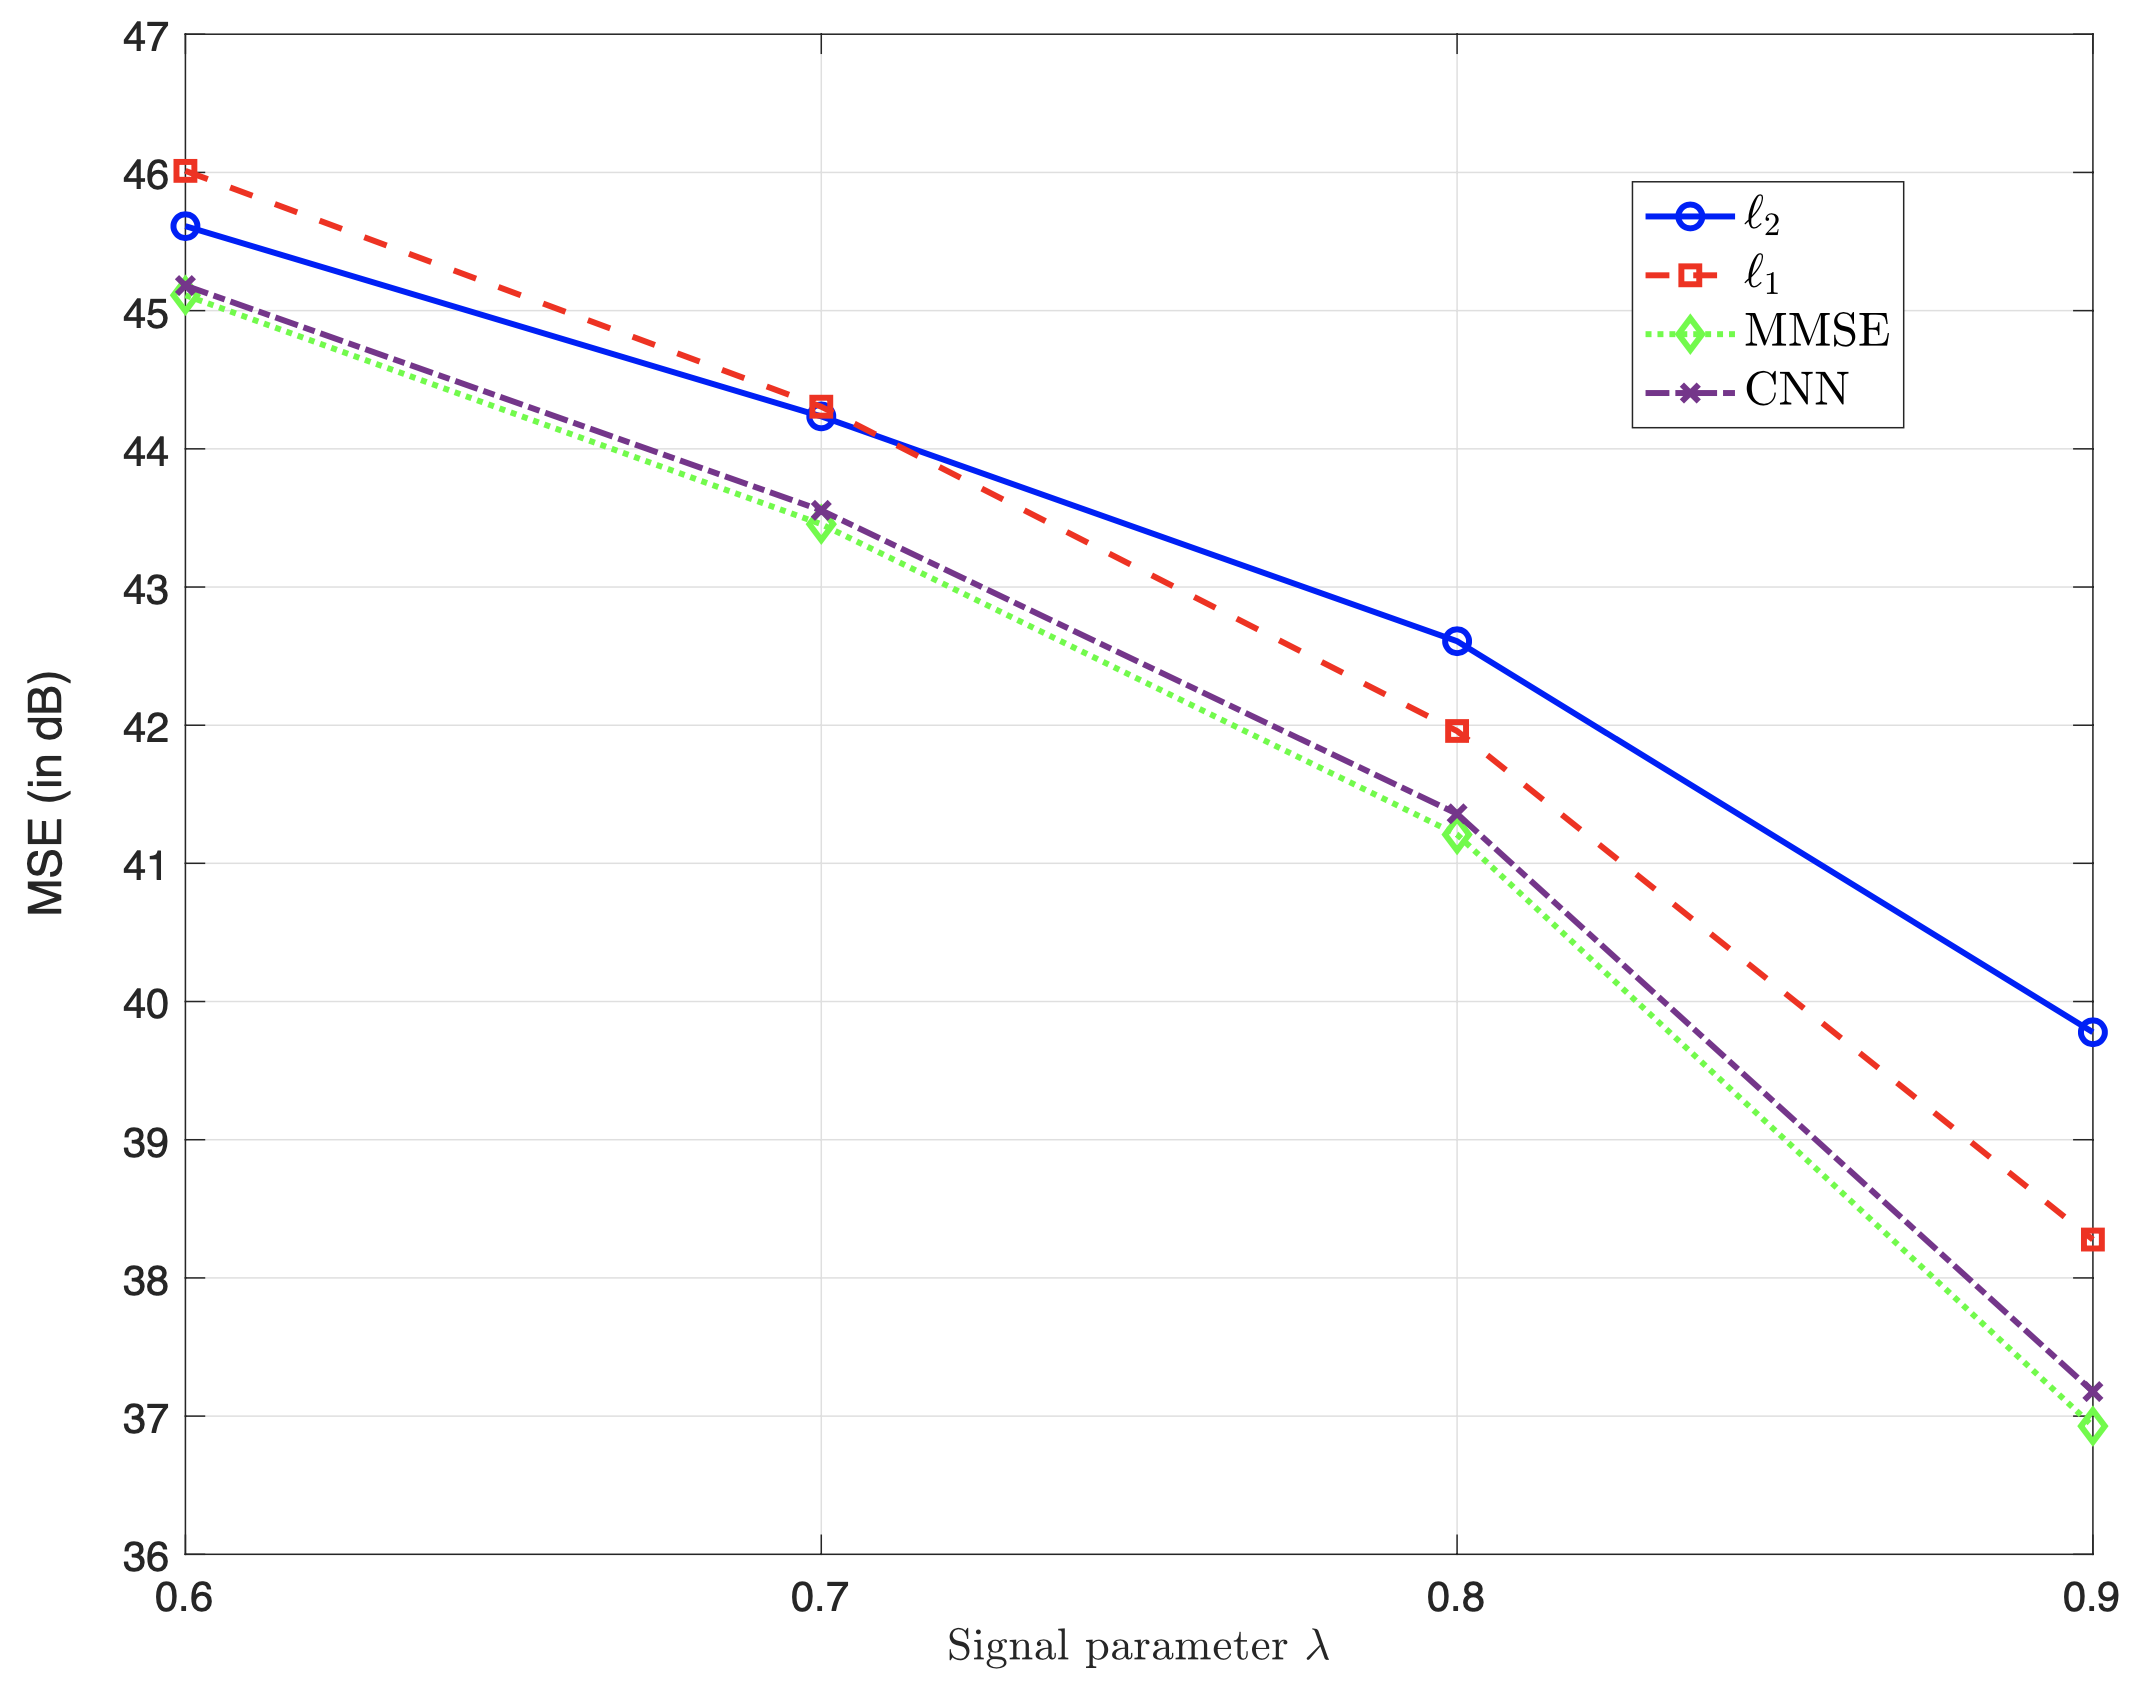
\includegraphics[width=\linewidth]{figures/deconvolution_bl}
    \caption{Deconvolution of L\'{e}vy processes with Bernoulli-Laplace increments.}
    \label{fig:deconvolution_bl}
\end{figure}


\subsection{Fourier Sampling}
Next, we look at a Fourier sampling problem which can be viewed as the one-dimensional equivalent of MRI. Here, the signal vector $\M s \in \R^{100}$ represents samples of a L\'{e}vy process associated with the Student's t distribution. In this case, the forward model $\M H$ resembles a discrete Fourier-like matrix (see Section \ref{sec:fourier_sampling_forward}). Thus, in order to construct $\M H$, we first sample $M' = 31$ rows (including the row for the DC component) of the DFT matrix. This selection is done in a quasi-random manner such that there is denser sampling at low frequencies. We then create the real system matrix $\M H: \R^{100} \rightarrow \R^{M}$, where $M = 2M' + 1$, by separating out the real and imaginary parts of each selected row from the DFT matrix. The Student's t distribution \eqref{eq:pdf_student} is parametrized by $\alpha$, which controls the tails of the distribution. Again, for chosen values of $\alpha$ and the AWGN variance $\sigma_n^{2}$, we create training, validation and test datasets with $50,000$, $1,000$ and $1,000$ samples, respectively.

The parameters for our CNN architecture are set as $F=3$, $C=32$ and $L=10$. Here, the initial estimate is $\widehat{\M s}_{0}(\M y) = (\M H^{T} \M y / M')$, and the CNN is trained for $500$ epochs with a learning rate of $10^{-4}$ and a batch size of $128$. The regularization parameters for the variational methods are determined in the same way as for the deconvolution experiments. For the MMSE estimator, the number of samples is $Q=15,000$ and the burn-in period is $B=5,000$.

We perform this Fourier sampling experiment for $\alpha \in \{1, 1.5, 2, 3, 10, 20 \}$. For each value of $\alpha$, the noise variance $\sigma_n^{2}$ is such that the (average) measurement SNR is around $40$ dB. The results for the test dataset are shown in Figure \ref{fig:fourier_sampling_student}.

The parameter $\alpha$ allows us to consider a very wide range of signals. As $\alpha \rightarrow \infty$, we approach the Gaussian regime. Thus, we observe that for larger values of $\alpha$, the $\ell_2$ estimator is optimal. On the other hand, $\alpha=1$ corresponds to the extremely heavy-tailed (sparse) Cauchy distribution. Consequently, as the value of $\alpha$ decreases, the relative performance of the $\ell_1$ estimator improves while that of the $\ell_2$ estimator deteriorates. For all the cases, the log estimator, which corresponds to a tunable MAP estimator for the Student's t distribution, attains the lowest MSE among the variational methods. Interestingly, the CNN-based method is near-optimal up to $\alpha = 2$, after which there seems to be a transition point and its performance drops sharply. In fact, for the extreme case of Cauchy signals, the CNN-based method performs worse than the $\ell_2$ estimator. A possible explanation for the poor performance of CNNs is that as the distribution becomes more heavy-tailed, the signals exhibit a vastly different range of values and this makes the training process very difficult.    

\begin{figure}[t]
    \centering
    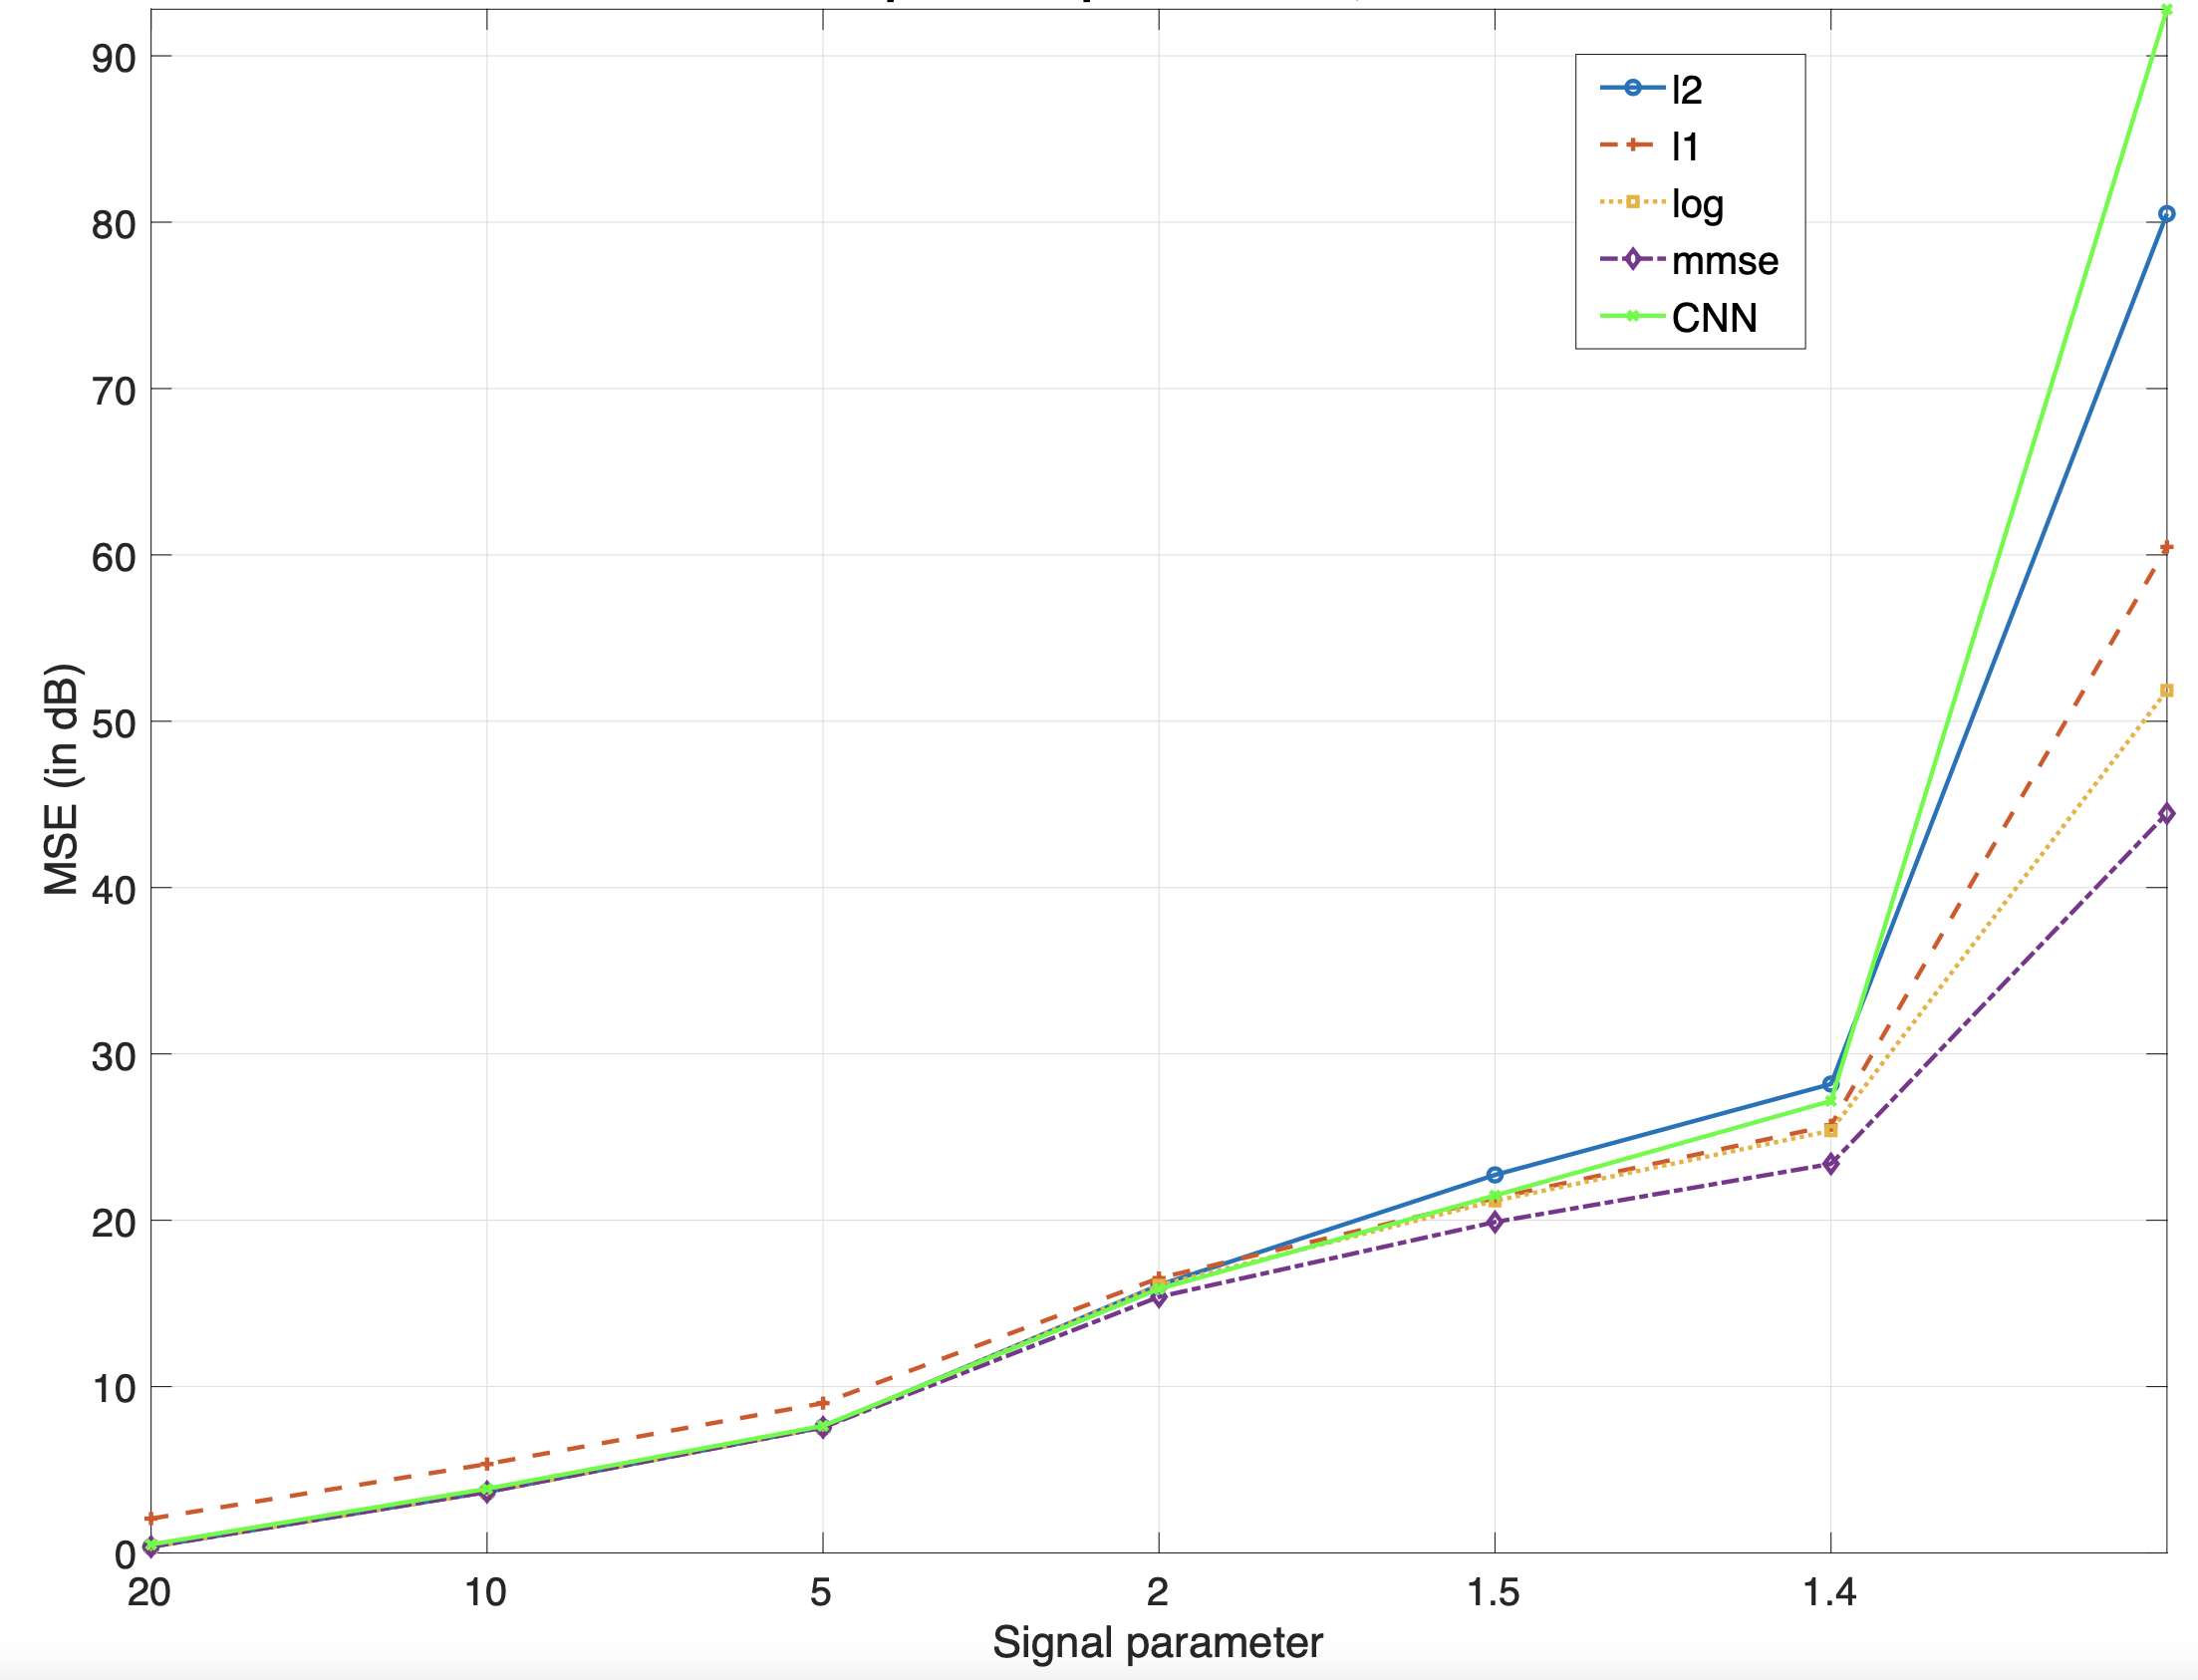
\includegraphics[width=\linewidth]{figures/fourier_sampling_student}
    \caption{Fourier Sampling of L\'{e}vy processes with Student's t increments.}
    \label{fig:fourier_sampling_student}
\end{figure}


\section{Conclusion}
    
    We have introduced a controlled environment for the objective study of
algorithms for linear inverse problems. We exemplified its potential on one of
the simplest categories of one-dimensional sparse stochastic processes
(L\'{e}vy processes), for which we derived the necessary tools--efficient
sampling schemes for the posterior distribution to obtain the MMSE estimator.
Despite this simplicity, our empirical results light on the fundamental
challenges of training the DnCNN model to remove artifacts in a simple Fourier
sampling reconstruction. Signals with heavy-tailed innovations will be very
poorly recovered and even the closed-form Tikhonov ($\ell_2$-regularized)
solution may perform better.


    
\section{Acknowledgements}

    We acknowledge access to the facilities and expertise of the CIBM Center
for Biomedical Imaging, a Swiss research center of excellence founded and
supported by Lausanne University Hospital (CHUV), University of Lausanne
(UNIL), École polytechnique fédérale de Lausanne (EPFL), University of
Geneva (UNIGE), and Geneva University Hospitals (HUG).

    
% \begin{itemize}
%     \item Deconvolution of Bernoulli-Laplace signals
%     \begin{itemize}
%         \item vary sparsity, 
%         \item $\ell_1$, $\ell_2$, log, MMSE, direct reconstruction CNN \\
%         CNNs perform close to MMSE in this setting
%         \item consider 2 settings: large number of training samples, low number of training samples. Maybe with infinite data also?
%         \item Compare direct CNN, unrolling, PnP (will be tough to do) \\
%         Maybe unrolling gives similar performance as direct CNNs but with fewer training data required (generalizes better).
%     \end{itemize}
%     \item Fourier sampling of student/alpha-stable signals
%     \begin{itemize}
%         \item vary sparsity
%         \item $\ell_1$, $\ell_2$, log, MMSE, direct reconstruction CNN \\
%         CNNs perform poorly in this setting
%         \item consider 2 settings: large number of training samples, low number of training samples. Maybe with infinite data also?
%         \item Compare direct CNN, unrolling, PnP (will be tough to do) \\
%         Maybe unrolling/PnP perform well due to their constrained nature
%     \end{itemize}
% \end{itemize}


\bibliographystyle{IEEEtran.bst} % use IEEEtran.bst style
\bibliography{refs}


\end{document}

